\chapter{Future Ideas for $HH\rightarrow \bbbb$}
\label{chap:future}

The searches presented in this thesis make use of a large suite of sophisticated techniques, selected 
through careful study and validation. During this process, a variety of interesting 
directions for the $HH\rightarrow b\bar{b}b\bar{b}$ analysis were explored by this thesis author, 
in collaboration with a few others\footnote{Notably Nicole Hartman (SLAC), who spearheaded much of the 
development and proof of concept work, in collaboration with Michael Kagan and Rafael Teixeira De Lima.}, 
but were not used due to a variety of constraints. We present two such interesting directions here, 
with the hope of encouraging further exploration of these techniques in future work.

\section{pairAGraph: A New Method for Jet Pairing}
As discussed in Chapter \ref{chap:bbbb}, one of the main problems to solve is the pairing of 
$b$-jets into Higgs candidates. Figure \ref{fig:pairing-massplanes} demonstrates that the choice 
of the pairing method, while important for achieving good reconstruction of signal events, also 
significantly impacts the structure of non-$HH$ events, leading to various biases in the 
background estimate. Evaluation of the pairing method therefore must take both of these factors 
into account. While we have presented some advantages in respective contexts for the pairing 
methods considered here, we of course would like to explore further improvements to this important 
component of the analysis.

To that end, we note that all of the pairing methods considered here share a common feature: 
four jets are selected, and the pairing is some discrimination between the available three pairings 
of these four jets. For the methods used in this analysis, the jet selection proceeds via a 
simple $p_{T}$ ordering, with $b$-tagged jets recieving a higher priority than non-tagged jets.

With the advent of a variety of machine learning methods for dealing with a variable number of 
inputs (e.g. recurrent neural networks~\cite{RNNs}, deep sets~\cite{DeepSets}, graph neural networks~\cite{GNNs}, 
and transformers~\cite{Transformers}), a natural place to improve on the 
pairing is to consider more than just four jets. The pairing and jet selection is then performed 
simultaneously, allowing for the incorporation of more event information in the pairing decision and 
the incorporation of jet correlation structure in the jet selection.

In practice, the majority of $HH\rightarrow\bbbb$ events have either four or five jets which pass 
the kinematic preselection, and any gain from this additional freedom would come from events with 
greater than or equal to five jets. However, this five jet topology is particularly exciting 
for scenarios such as events with initial state radiation (ISR), in which the $HH->4b$ jets are offset by 
a single jet with $p_{T}$ similar in magnitude to that of the $HH->4b$ system. Such events have explicit 
event level information which is not encoded with the inclusion of only the $HH->4b$ jets, and are 
pathological if the ISR jet happens to pass $b$-tagging requirements.

Additionally, with the use of lower tagged regions for background estimation and alternate 
signal regions, this extra flexibility in jet selection may provide a very useful bias -- 
since the algorithm is trained on signal, the selected jets for the pairing will be the 
most ``4b-like'' jets available in the considered set.

For the studies considered here, a transformer~\cite{Transformers} based architecture is used. This is 
best visualized by considering the event as a graph with jets corresponding to nodes and 
edges corresponding to potential connections -- for this reason, we term this algorithm ``pairAGraph''.
The approach is as follows: each jet, $i$, is represented by some vector of input variables, 
$\vec{x}_i$, in our case the four-vector information, $(p_{T}, \eta, \phi, E)$ of each jet, plus 
information on the $b$-tagging decision. A multi-layer perceptron (MLP) is used to create a latent 
embedding, $\mathbf{h}(\vec{x}_i)$, of this input vector.

To describe the relationship between various jets in the event, we then define a vector $\vec{z}_{i}$ 
for each jet as 
\begin{equation}
\vec{z}_i = \sum\limits_j w_{ij}\mathbf{h}(\vec{x}_j)
\end{equation}
where $j$ runs over all jets in the event (including $i=j$), the $w_{ij}$ can be thought of as 
edge weights, and $\mathbf{h}(\vec{x}_j)$ is the latent embedding for jet $j$ mentioned above.

Within this formula, both $\mathbf{h}$ and the $w_{ij}$ are learnable. To learn an appropriate 
latent mapping and set of edge weights, we define a similarity metric corresponding to each 
possible jet pairing:
\begin{equation}
\vec{z}_{1a}\cdot \vec{z}_{1b} + \vec{z}_{2a}\cdot \vec{z}_{2b}
\end{equation}
where subscripts $1a$ and $1b$ correspond to the two jets in pair 1, $2a$ and $2b$ to 
the jets in pair 2 for a given pairing of four distinct jets.

This similarity metric is calculated for all possible pairings, which are then passed through a 
softmax~\cite{Softmax} activation function, which compresses these scores to between $0$ and $1$ 
with sum of $1$, lending an interpretation as probability of each pairing.

In training, the ground truth pairing is set by \emph{truth matching} jets to the $b$-jets 
in the $HH$ signal simulation -- a jet is considered to match if it is $< 0.3$ in $\Delta R$
away from a $b$-jet in the simulation record. Given this ground truth, a cross-entropy loss \todo{cite}
is used on the softmax outputs, and $w_{ij}$ and $\mathbf{h}$ are updated correspondingly.
Training in such a way corresponds to updating $w_{ij}$ and $\mathbf{h}$ to maximize the similarity 
metric for the correct pairing.

In evaluation, the pairings with a higher score (and therefore higher softmax output) given 
the trained $h$ and $w_{ij}$ therefore correspond to the pairings that are most ``HH-like''. 
The maximum over these scores is therefore the pairing used as the predicted result from 
the algorithm.

Because the majority of $HH\rightarrow\bbbb$ events have either four or five jets, it was 
found to be sufficient to only consider a maximum of 5 jets. Consideration of more is in 
principle possible, but the quickly expanding combinatorics leads to a rapidly more 
difficult problem. The jets considered are the five leading jets in $p_{T}$. Notably, 
this set of jets may include jets which are not $b$-tagged, even for the nominal $4b$ 
region -- therefore events with $4$ $b$-tagged jets are not required to use all of them 
in the construction of Higgs candidates, in contrast to the other algorithms used in this 
thesis.

A comparison of the pairAGraph jet selection with the baseline selection used in Chapter ~\ref{chap:bbbb} 
is considered in Table \ref{tbl:pag-jet-sel} for the MC16a Standard Model non-resonant signal. As a reminder, 
the baseline selection orders jets by $p_{T}$, selecting first the highest $p_{T}$ $b$-tagged jets (according 
to the $b$-tag region definition) and then the highest $p_{T}$ non-tagged jets. The first four jets 
in this ordering are used. 

For the comparison presented in Table \ref{tbl:pag-jet-sel}, only the leading five jets are considered in 
applying both algorithms in order to compare results on more equal footing. The numbers shown are the percent 
of the time that the correct jets are selected for the Higgs candidates by each algorithm, given that the 
correct jets fall within these leading five jets, where ``correct'' here means truth matched to the 
corresponding $b$-quarks. pairAGraph demonstrates a slight improvement over the baseline for $4b$, which widens when 
considering lower $b$-tag categories. Given that four $b$-quarks are present in all of these 
categories, this suggests that pairAGraph is able to recover information in the case of, e.g., mis-tagged 
jets.

\begin{table}
\centering
\begin{tabular}{|c | c | c|}
\hline
\textbf{4b correct jets} & 96.7\% & 96.0\%\\
\hline
\textbf{3b+1 loose correct jets} & 96.3\% & 95.2\%\\
\hline
\textbf{3b correct jets} & 91.6\% & 83.2\%\\
\hline
\end{tabular}
\caption{\label{tbl:pag-jet-sel} Percent of the time that the correct jets are selected for the 
Higgs candidates by each algorithm, given that the correct jets fall within the set of considered jets,  
where ``correct'' here means truth matched to the corresponding $b$-quarks. Only the leading five jets 
are considered in the assessment of both algorithms. Definitions of the $4b$ and $3b+1$ loose categories 
are as described in Section \ref{sec:analysis-selection}, where $3b$ requires three $b$-tagged jets and 
the fourth jet is untagged. pairAGraph demonstrates a slight improvement over the 
baseline for $4b$, which widens when considering lower $b$-tag categories. Given that four $b$-quarks are present 
in all of these categories, this suggests that pairAGraph is able to recover information in the case of, 
e.g., mis-tagged jets.}
\end{table}


Table \ref{tbl:pag-accuracy} compares the $HH$ pairing accuracy of a few different pairing algorithms for the 
Standard Model signal. Notably, pairAGraph demonstrates a higher pairing accuracy immediately after paring, 
but all methods are quite comparable after the full analysis selection.
\begin{table}
\centering
\begin{tabular}{|c | c | c|}
\hline
&\textbf{After Pairing} & \textbf{After Full Selection}\\
\hline \hline
$D_{HH}$ & 71.8\% & 93.6\% \\
\hline
$\min{\Delta R}$ & 69.7\% & 94.7\% \\
\hline
pairAGraph & 78.4\% & 94.2\%\\
\hline
\end{tabular}
\caption{\label{tbl:pag-accuracy} Pairing accuracy evaluated for the Standard Model signal (MC16a), comparing 
$D_{HH}$ and $\min{\Delta R}$ (discussed in Chapter \ref{chap:bbbb}) with pairAGraph trained on the Standard Model 
signal. Numbers are shown both immediately after pairing and after the full analysis selection. pairAGraph demonstrates 
a 7-8\% higher accuracy than the other algorithms immediately after pairing, but all methods are quite comparable after 
the full analysis selection.}
\end{table}

As mentioned in Chapter \ref{chap:bbbb}, though the pairing is quite important for signal events, it also 
must be applied to events in data, where the overwhelming majority of events do not contain $HH$. Though in 
general, pairing methods select for an $HH$-like topology, the additional flexibility of pairAGraph to 
choose which jets enter the candidate $HH$ system provides an additional handle to shape the 
kinematics of events in data. Examples of this impact are seen in Figures \ref{fig:no-rw-pt-hh-compare} and 
\ref{fig:pt-hh-compare}, which compare the $2b$ and $4b$ distributions of $p_{T}$ of the $HH$ candidate 
system between BDT pairing and pairAGraph pairing before and after reweighting. $HH$ $p_{T}$ was 
chosen as it is a variable which demonstrates both a large difference between $2b$ and $4b$ and 
a residual mis-modeling after reweighting. As can be seen in Figure \ref{fig:no-rw-pt-hh-compare}, 
the $2b$ and $4b$ distributions are more similar before reweighting with pairAGraph. Figure \ref{fig:pt-hh-compare} 
further shows that the residual mis-modeling after reweighting is reduced, along with the corresponding uncertainty. 
While this is not fully conclusive, it provides a hint that the jets chosen for the $2b$ event $HH$ candidate 
system may be more ``$4b$-like'' than the jets chosen with the baseline selection.

\begin{figure}[ht]
	\centering
	\subfloat[BDT Paring]{\label{fig:no-rw-BDT-pt-hh}%
		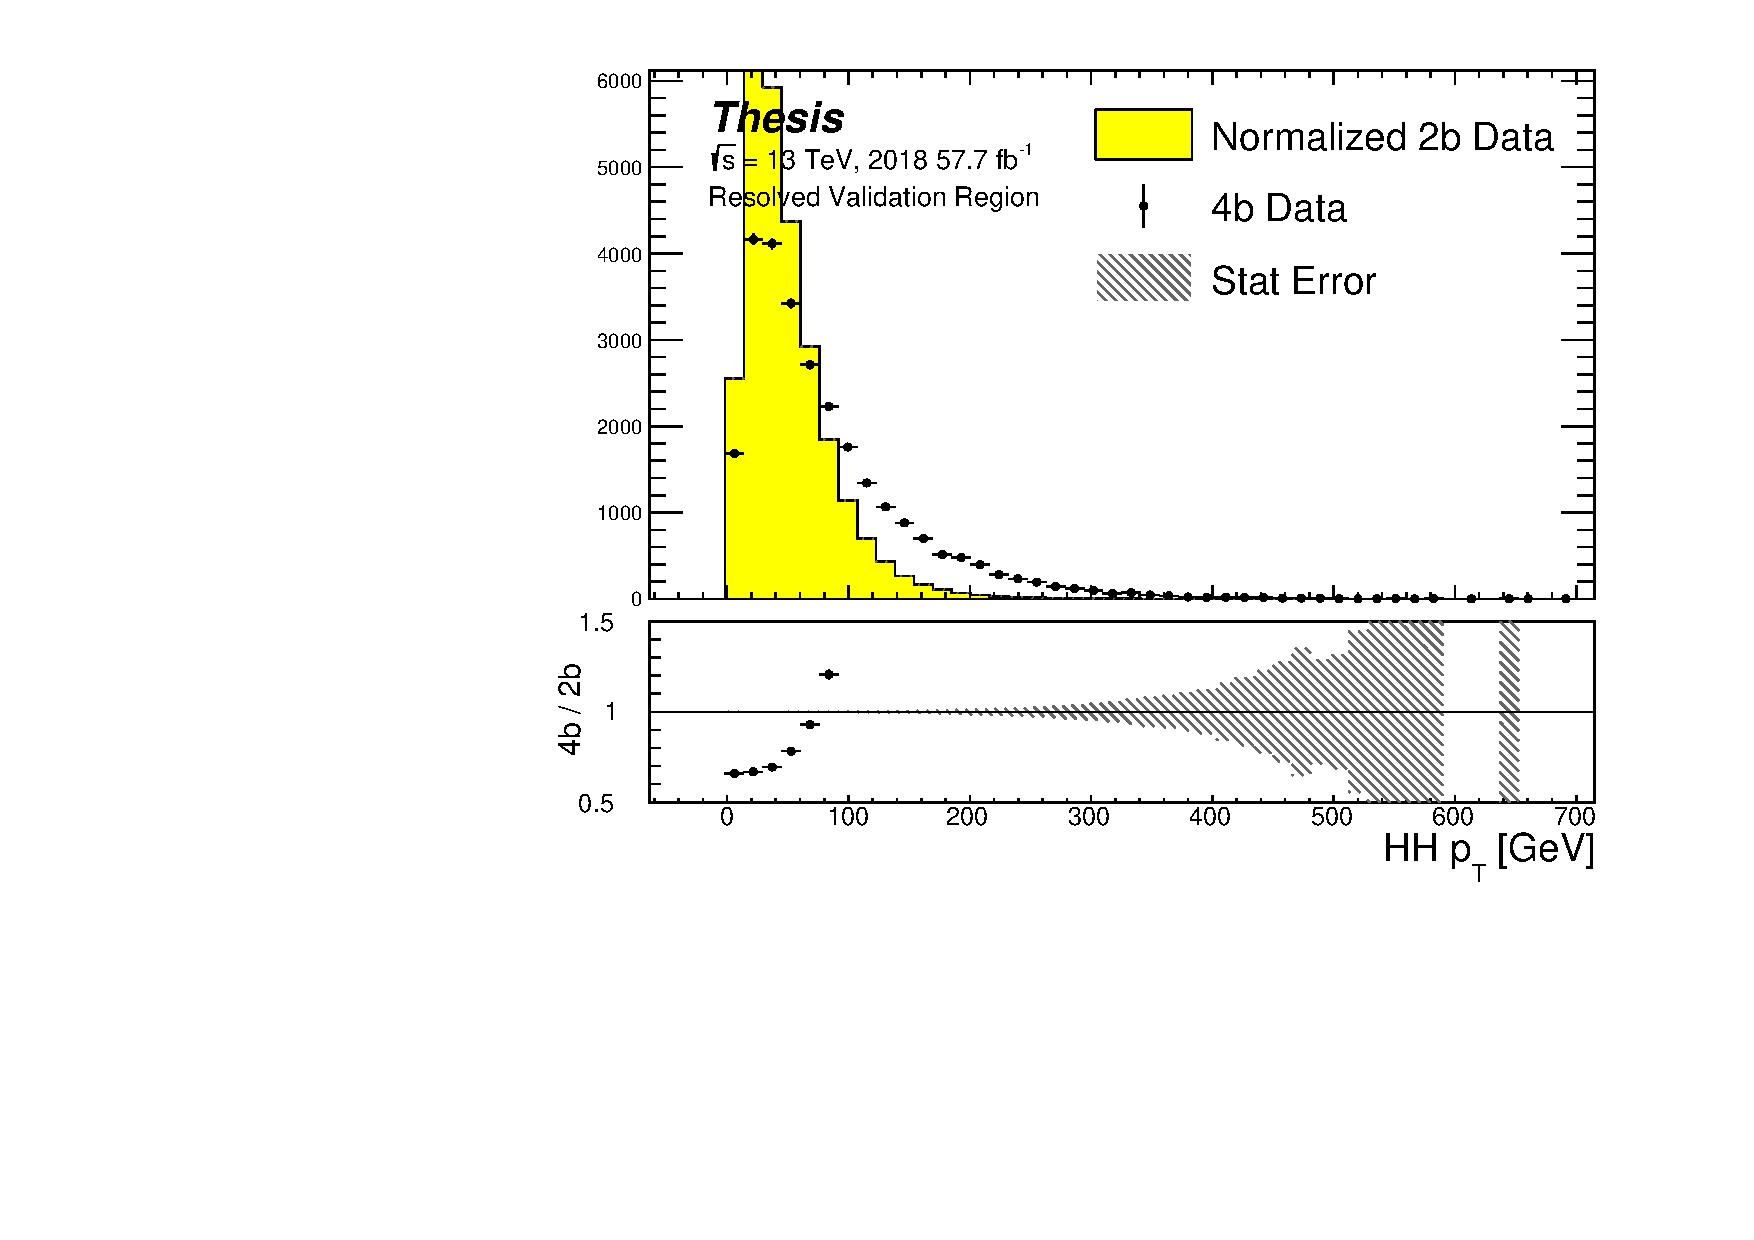
\includegraphics[width=0.48\textwidth]{figures/thesis-pt-hh-norw-bstrap-med-Validation-NN-18.pdf}
	}
	\subfloat[pairAGraph]{\label{fig:no-rw-PAG-pt-hh}%
		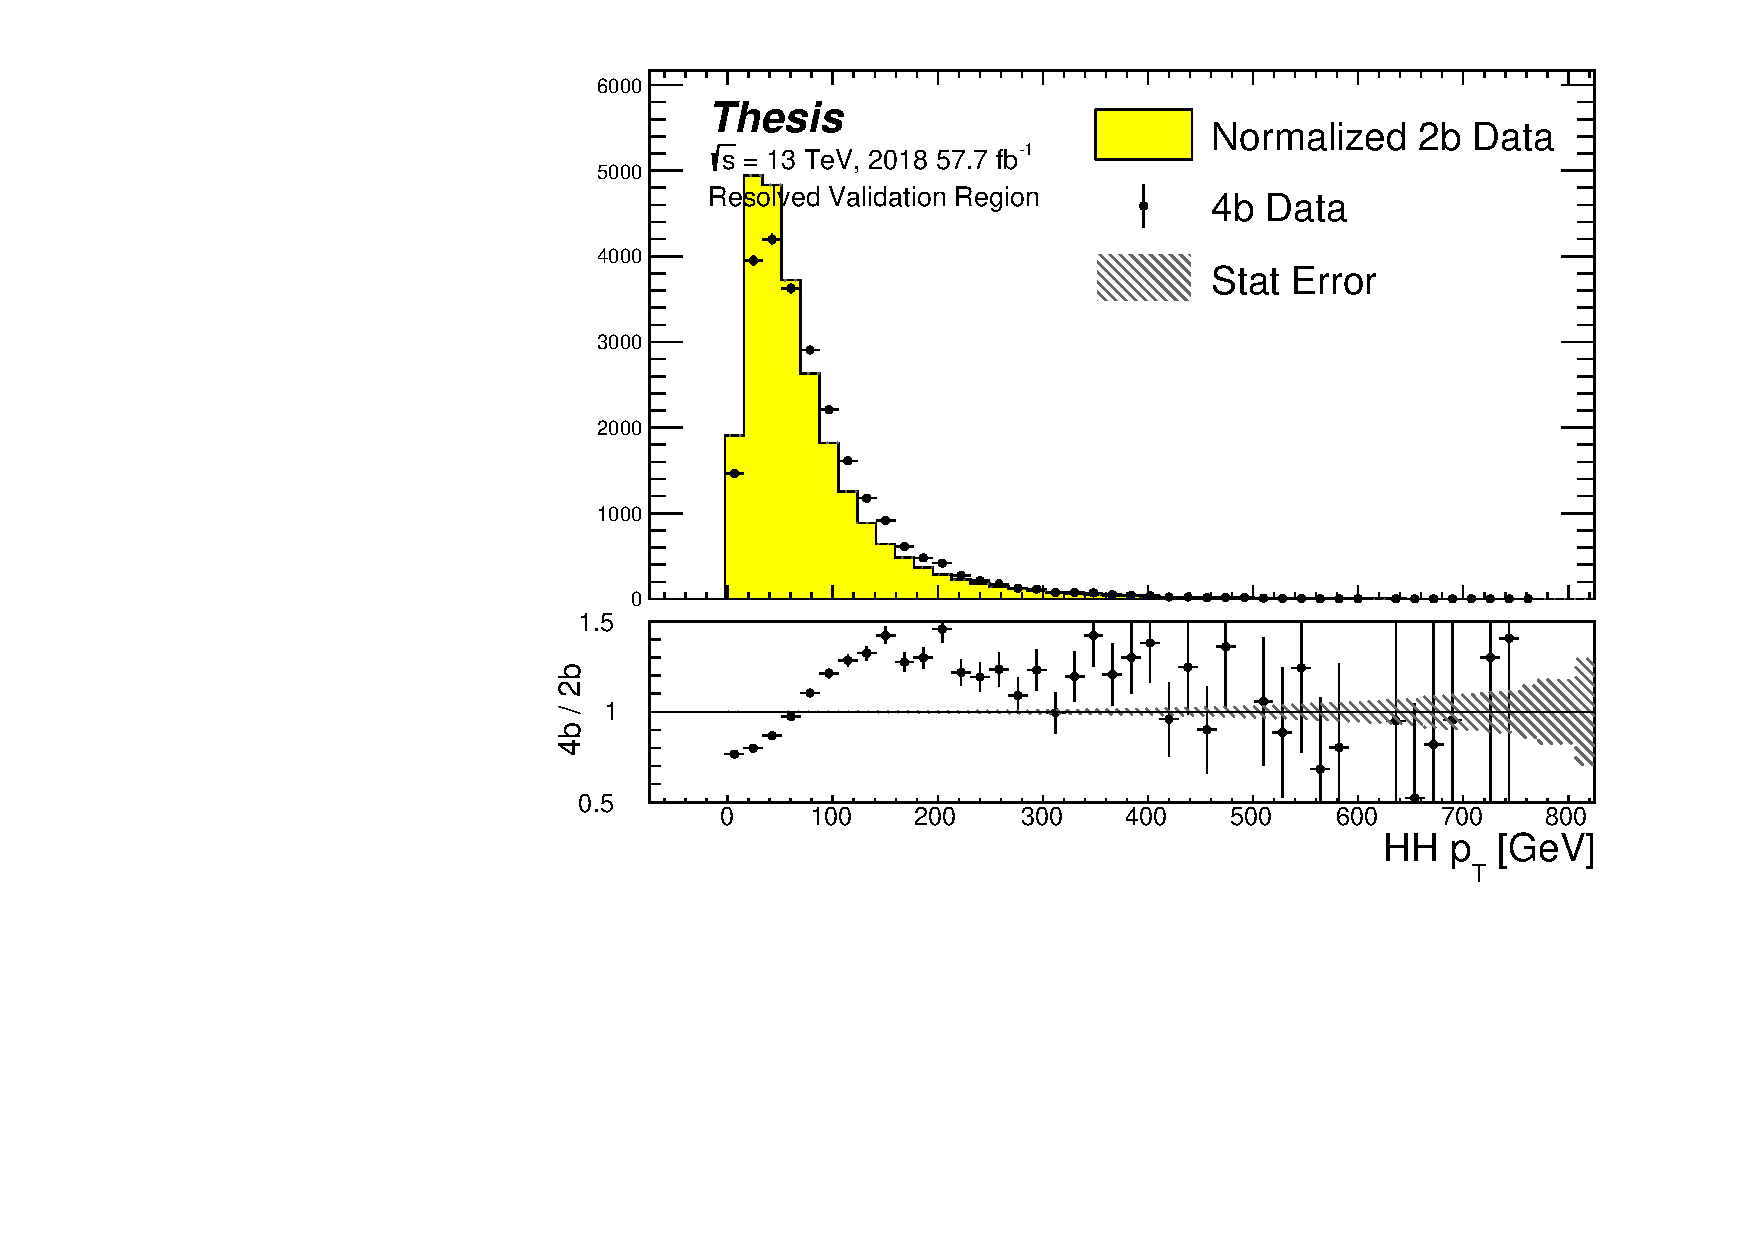
\includegraphics[width=0.48\textwidth]{figures/thesis-PAG-pt-hh-norw-bstrap-med-Validation-NN-18.pdf}
	}
	\caption{\label{fig:no-rw-pt-hh-compare} Comparison of distributions of $HH$ $p_{T}$ in the 2018 resonant validation region before reweighting for BDT pairing (left) and pairAGraph (right). $HH$ $p_{T}$ is a variable with a 
	large difference between $2b$ and $4b$, but the relative shapes seem to be more similar for pairAGraph than 
	for BDT paring, corresponding to the hypothesis that pairAGraph chooses more ``$4b$-like'' jets.}
\end{figure}


\begin{figure}[ht]
	\centering
	\subfloat[BDT Paring]{\label{fig:BDT-pt-hh}%
		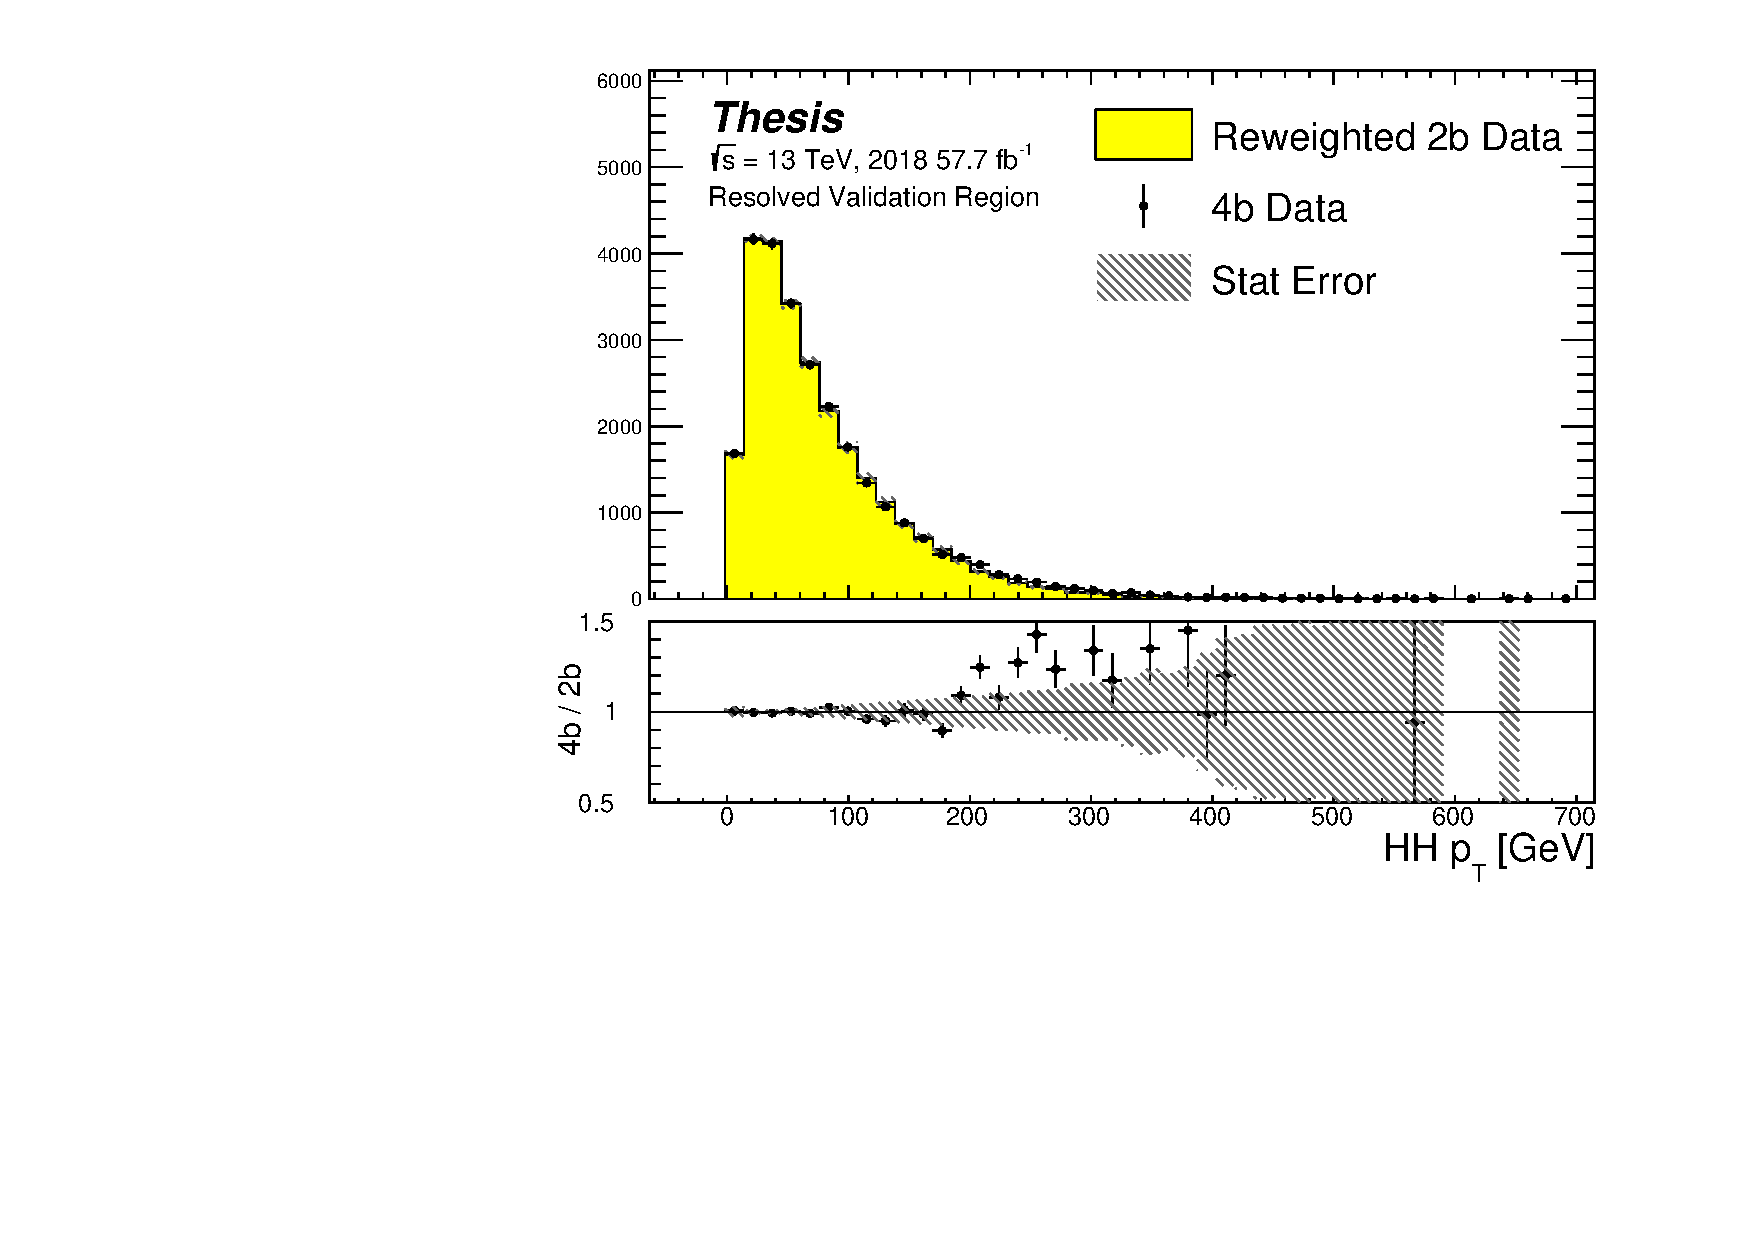
\includegraphics[width=0.48\textwidth]{figures/thesis-pt-hh-bstrap-med-Validation-NN-18.pdf}
	}
	\subfloat[pairAGraph]{\label{fig:no-rw-PAG-pt-hh}%
		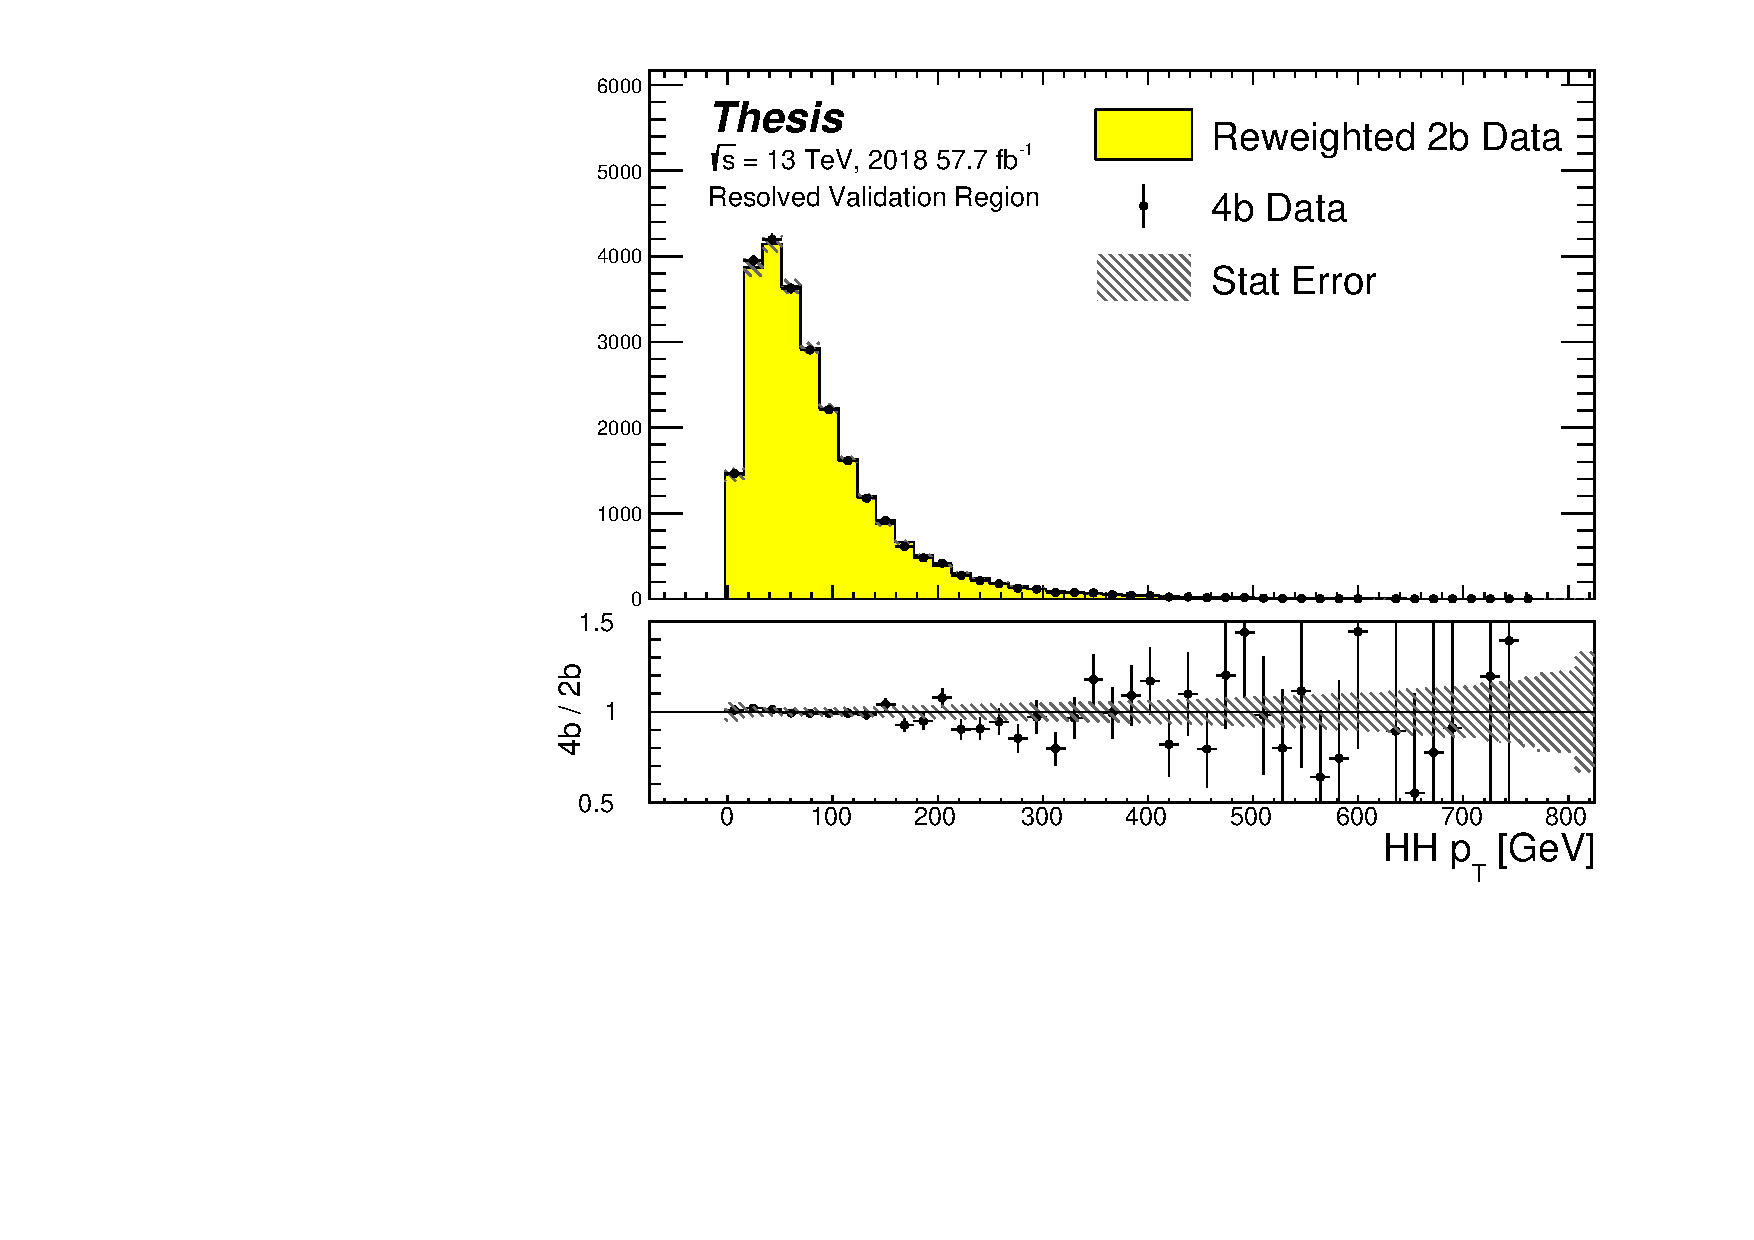
\includegraphics[width=0.48\textwidth]{figures/thesis-PAG-pt-hh-bstrap-med-Validation-NN-18.pdf}
	}
	\caption{\label{fig:pt-hh-compare} Comparison of distributions of $HH$ $p_{T}$ in the 2018 resonant validation region after reweighting for BDT pairing (left) and pairAGraph (right). $HH$ $p_{T}$ is a variable with a 
	large difference between $2b$ and $4b$, and the reweighted agreement in the high $p_{T}$ tail is significantly 
	improved with pairAGraph, with a corresponding reduction in the assigned bootstrap uncertainty in that region.}
\end{figure} 


\section{Background Estimation with Mass Plane Interpolation}
The choice of a pairing algorithm that results in a smooth mass plane (such as $\min{\Delta R}$) 
opens up a variety of options for the background estimation. While the method based on 
reweighting of $2b$ events used for this thesis performs well and has been extensively 
studied and validated, it also relies on several assumptions. In particular, the reweighting is derived 
between e.g., $2b$ and $4b$ events \emph{outside} of the signal region and then applied to $2b$ 
events \emph{inside} the signal region, with the assumption that the $2b$ to $4b$ transfer function 
will be sufficiently similar in both regions of the mass plane. An uncertainty is assigned to 
account for the bias due to this assumption, but the extrapolation in the mass plane is never 
explicitly treated in the nominal estimate. While the approach of reweighting $2b$ events within the 
signal region does have the advantage of incorporating explicit signal region information (that is, 
the $2b$ signal region events), the importance of the extrapolation bias motivates consideration 
of a method that operates within the $4b$ mass plane. This additionally removes the reliance on lower 
$b$-tagging regions, allowing for the use of, e.g. $3b$ triggers, and future-proofing the analysis 
against trigger bandwidth constraints in the low tag regions.

The pairAGraph pairing method discussed in the previous section was developed concurrently with 
these studies and demonstrates good properties for an interpolated estimate (as shown below), and 
is therefore used in the following.

The method considered here relies on the following: for a given vector of 
input variables (event kinematics, etc), $\vec{x}$, the joint probability in the $HH$ mass 
plane may be written as:
\begin{equation}
p(\vec{x}, m_{H1}, m_{H2}) = p(\vec{x}| m_{H1}, m_{H2})p(m_{H1}, m_{H2})
\end{equation}
by the chain rule of probability. This means that the full dynamics of events 
in the $HH$ mass plane may be described by (1) the conditional probability of 
considered variables $\vec{x}$, given values of $m_{H1}$ and $m_{H2}$, and (2) the 
density of the mass plane itself. 

We present here an approach which uses normalizing flows~\cite{NormalizingFlows} to model the 
conditional probabilities of events in the mass plane and Gaussian processes to 
model the mass plane density. These models are trained in a region around, but not 
including, the signal region, and the trained models are then used to construct an 
\emph{interpolated} estimate of the signal region kinematics. This approach therefore 
explicitly treats event behavior within the mass plane, avoiding the concerns associated 
with a reweighted estimate. Validation of such a method, as well as assessing of closure and 
biases of the method, may be done in alternate $b$-tagging or kinematic regions, notably the 
now unused $2b$ region, results of which are shown below.

\subsection{Normalizing Flows}
Normalizing flows model observed data $x\in X$, with $x \sim p_{X}$, as the output of an 
invertible, differentiable function $f: X \rightarrow Z$, with $z\in Z$ a latent 
variable with a simple prior probability distribution (often standard normal), $z\sim p_{Z}$. 
From a change of variables, given such a function, we may write
\begin{equation}
p_{X}(x) = p_{Z}(f(x))\qty|\det\qty(\frac{d(f(x))}{dx})|
\end{equation}
where $\qty(\frac{d(f(x))}{dx})$ is the Jacobian of $f$ at $x$.

The problem of normalizing flows then reduces to (1) choosing sets of $f$ which are 
both tractable and sufficiently expressive to describe observed data, and (2) optimizing 
associated sets of functional parameters on observed data via maximum likelihood esitmation 
using the above formula. Sampling from the learned density is done by drawing from the 
latent distribution $z\sim p_Z$ (cf. inverse transform sampling) -- the corresponding 
sample is then $x\sim p_X$ with $x=f^{-1}(z)$.

A standard approach to the definition of these $f$ is as a composition of affine transformations (e.g. 
RealNVP~\cite{RealNVP}), 
that is, transformations of the form $\alpha z + \beta$, with $\alpha$ and $\beta$ learnable 
parameter vectors. This can roughly be though of as shifting and squeezing the input
input prior density in order to match the data densitiy. However, this has somewhat limited expressivity, 
for instance in the case of a multi-modal density.

This work thus instead relies on neural spline flows~\cite{NeuralSplineFlows} 
in which the functions considered are monotonic rational-quadratic splines, which have an analytic inverse.
A rational quadratic function has the form of a quotient of two quadratic polynomials, namely,
\begin{equation}
f_j(x_i) = \frac{a_{ij} x_i^2 + b_{ij} x_{ij} + c_{ij}}{d_{ij}x_i^2 + e_{ij} x_i + f_{ij}}
\end{equation}
with six associated parameters ($a_{ij}$ through $f_{ij}$) per each piecewise bin $j$ of the spline and 
each input dimension $i$. This is explicitly more flexible and expressive than a simple affine 
transformation, allowing, e.g., the treatment of multi-modality via the piecewise nature of the spline. 

The rational quadratic spline is defined on an set interval. The transformation outside of this interval 
is set to the identity, with these linear tails allowing for unconstrained inputs. The boundaries between 
bins of the spline are set by coordinates scalled \emph{knots}, with $K+1$ knots for $K$ bins -- the two 
endpoints for the spline interval plus the $K-1$ internal boundaries. The derivatives 
at these points are constrained to be positive for the internal knots, and boundary 
derivatives are set to 1 to match the linear tails. 

The bin widths and heights are learnable ($2\cdot K$ parameters) as are the internal knot derivatives
($K-1$ parameters), and these $3K-1$ ouputs of the neural network are sufficient to define a monotonic 
rational-quadratic spline which passes through each knot and has the given derivative value at each knot.

In the context of the $HH\rightarrow 4b$ analysis, a neural spline flow is used to model the four vector 
information of each Higgs candidate, conditional on their respective masses. The resulting flow is 
therefore five dimensional, with inputs $x$ = ($p_{T, H1}$, $p_{T, H2}$, $\eta_{H1}$, $\eta_{H2}$, 
$\Delta\phi_{HH}$), where the ATLAS $\phi$ symmetry has been encdoded by assuming $\phi_{H1} = 0$. 
Conditional variables $m_{H1}$ and $m_{H2}$ are not modeled by the flow, but ``come along for the ride''. 
A standard normal distribution in $5$ dimensions is used for the underlying prior. Modeling of the four 
vectors was chosen in order to reduce bias from modeling $m_{HH}$ directly.

The trained flow model then gives a model for $p(x|m_{H1}, m_{H2})$ which may be sampled from to reconstruct 
distributions of $HH$ kinematics given values of $m_{H1}$ and $m_{H2}$.

\subsection{Gaussian Processes}
The second piece of this background estimate is the modeling of the mass plane density, $p(m_{H1}, m_{H2})$. 
This is done using Gaussian process regression -- note that a similar procedure is used to define a systematic 
in the boosted $4b$ analysis. Generally, Gaussian processes are a collection of random variables in which every 
finite collection of said variables is distributed according to a multivariate normal distribution. For the 
context of Gaussian process regression, what we consider is a Gaussian process over function space, that is, 
for a collection of points, $x_{1}, \ldots, x_{N}$, the space of corresponding function 
values, $(f(x_{1}), \ldots, f(x_{N}))$ is Gaussian process distributed, that is, described by an $N$ dimensional 
normal distribution with mean $\mu$, covariance matrix $\Sigma$.

For a single point, this would correspond to a function space described entirely by a normal distribution, 
with various samples from that distribution yielding various candidate functions. For multiple points, a 
covariance matrix describes the relationship between each pair of points -- correspondingly, it is represented 
via a \emph{kernel function}, $K(x, x')$. As, in practice, $\mu$ may always be set to 0 via a centering of the 
data, the kernel function fully defines the considered family of functions.

The considered family of functions describes a Bayesian \emph{prior} for the data. This prior may be conditioned 
on a set of training data points $(X_{1}, \vec{y}_1)$. This conditional \emph{posterior} may then be used to make 
predictions $\vec{y}_2 = f(X_2)$ at a set of new points $X_2$. Because of the Gaussian process prior assumption, 
$\vec{y}_1$ and $\vec{y}_2$ are assumed to be jointly Gaussian. We may therefore write
\begin{equation}
\begin{pmatrix}\vec{y}_1 \\ \vec{y}_2\end{pmatrix} \sim 
\mathcal{N}\begin{pmatrix}\begin{pmatrix}0\\0 \end{pmatrix}, 
\begin{pmatrix}K(X_1, X_1) & K(X_1, X_2)\\ K(X_1, X_2) & K(X_2, X_2)\end{pmatrix}\end{pmatrix}
\end{equation}
where we have used that the kernel function is symmetric and assumed prior mean 0. 

By standard conditioning properties of Gaussian distributions, 
\begin{equation}
\vec{y}_2 | \vec{y}_1 \sim \mathcal{N}(K(X_2, X_1)K(X_1,X_1)^{-1}\vec{y}_1, K(X_2, X_2)-K(X_2,X_1)K(X_1,X_1)^{-1}K(X_1, X_2))
\end{equation}
which is the sampling distribution for a Gaussian process given kernel $K$. In practice, the 
mean of this sampling distribution is used as the function estimate, with an uncertainty from the
predicted variance at a given point.

The choice of kernel function has a very strong impact on the fitted curve, and must therefore be chosen to 
express the expected dynamics of the data. A common such choice is a radial basis function (RBF) kernel, which 
takes the form
\begin{equation}
K(x, x') = \exp\qty(-\frac{d(x, x')^2}{2l^2})
\end{equation}
where $d(\cdot, \cdot)$ is the Euclidean distance and $l > 0$ is a length scale parameter. Conceptually, 
as distances $d(x, x')$ increase relative to the chosen length scale, the kernel smoothly dies off -- 
further away points influence each other less. 

Coming back to our case of the mass plane, the procedure runs as follows:
\begin{enumerate}
	\item A binned 2d histogram of the blinded mass plane is created in a window 
	around the ``standard'' analysis regions. Bins which have any overlap with the 
	signal region are excluded.
	\item A Gaussian process is trained using the bin centers, values as training points. 
	The scikit-learn implementation~\cite{scikit-learn} is used, with RBF kernel with anisotropic length scale 
	($l$ is dimension 2).  The length scale is initialized to $(50, 50)$ to cover the signal region, 
	and optimized by minimizing the negative log-marginal likelihood on the training data, 
	$-\log p(\vec{y}|\theta)$. Training data is centered and scaled to mean $0$, variance $1$, 
	and a statistical error is included in the fit.
	\item The Gaussian process is then used to predict the density $p(m_{H1}, m_{H2})$ in the signal region. 
	This may then be sampled from via an inverse transform sampling to generate values $(m_{H1}, m_{H2})$ 
	according to the density (specifically, according to the mean of the Gaussian process posterior). 
	Though in principle the Gaussian process sampling is not limited 
	to bin centers, this is kept for simplicity, with a uniform smearing applied within each 
	sampled bin to approximate the contiuous estimate, namely, if a bin is sampled from, the 
	returned value is drawn uniformly at random within the sampled bin. 
	\item The sampling in the previous step can be arbitrary -- to set the overall normalization, 
	a Monte Carlo sampling of the Gaussian process is done to approximate the relative fraction 
	of events predicted both inside ($f_{in}$) and outside ($f_{out}$) of the signal region, within 
	the training box. The number of events outside of the signal region ($n_{out}$) is known, therefore, 
	the number of events inside of the signal region, $n_{in}$, may be estimated as 
	\begin{equation}
	n_{in} = \frac{n_{out}}{f_{out}}\cdot f_{in}.
	\end{equation}
	Note that the Monte Carlo sampling procedure is simply a set of samples of the Gaussian 
	process from uniformly random values of $m_{H1}, m_{H2}$, and is the most convenient 
	approach given the irregular shape of the signal region.
\end{enumerate}
This procedure results in a generated set of predicted $m_{H1}, m_{H2}$ values for signal region
background events, along with an overall yield prediction.

\subsection{The Full Prediction}
Given the normalizing flow parametrization of $p(x | m_{H1}, m_{H2})$ and the Gaussian process generation of 
$(m_{H1}, m_{H2}) \sim p(m_{H1}, m_{H2})$ and prediction of the signal region yield, all of the pieces are 
in place to construct an interpolation background estimate. Namely
\begin{enumerate}
	\item Gaussian process sampled $(m_{H1}, m_{H2})$ values are provided to the normalizing flow to predict 
	the other variables for the Higgs candidate four-vectors. These are used to construct the $HH$ system (notably 
	$m_{HH}$).
	\item These final distributions are normalized according to the predicted background yield.
\end{enumerate}

\subsection{Results}
All of the following results use the pairAGraph pairing algorithm, and reweighted results use the region 
definitions from the resonant analysis.

The Gaussian process sampling procedure is trained on a small fraction ($0.01$) of $2b$ data to mimic 
the available $4b$ statistics. This fraction of $2b$ data is blinded, and the prediction of the estimate trained on 
this blinded region may then be compared to real $2b$ data in the signal region. The 
predictions for signal region $m_{H1}$ and $m_{H2}$ individually are shown in 
Figure \ref{fig:gp-marginals-18}, and the resulting mass planes are compared in Figure \ref{fig:gp-massplane-18}.  Good agreement is seen.
\begin{figure}[ht]
	\centering
	\subfloat{\label{fig:gp-mh1-18}%
		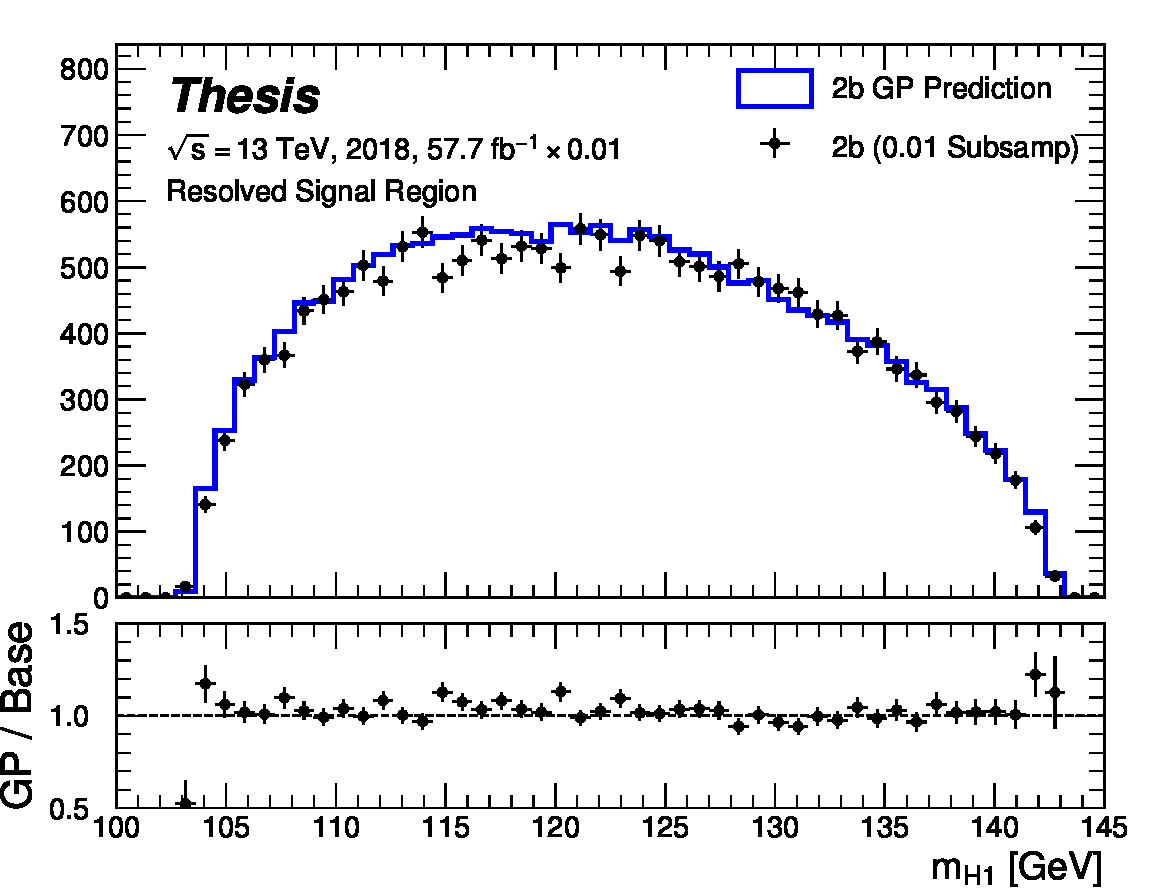
\includegraphics[width=0.48\textwidth]{figures/thesis-pure2b-GP-vs-real2b-0.01subsamp-2018-Signal-m-h1.pdf}
	}
	\subfloat{\label{fig:gp-mh2-18}%
		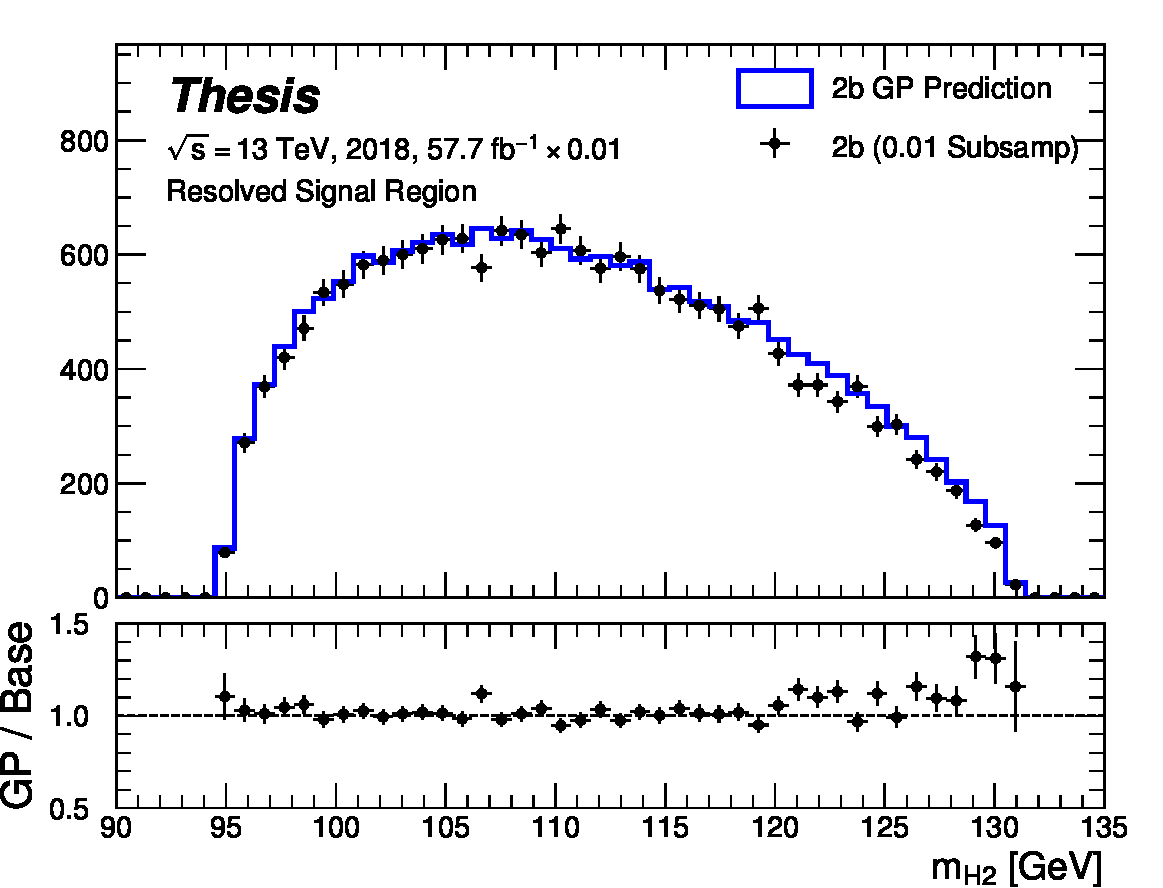
\includegraphics[width=0.48\textwidth]{figures/thesis-pure2b-GP-vs-real2b-0.01subsamp-2018-Signal-m-h2.pdf}
	}
	\caption{\label{fig:gp-marginals-18} Gaussian process sampling prediction of marginals $m_{H1}$ and $m_{H2}$ 
	for $2b$ signal region events compared to real $2b$ signal region events for the 2018 dataset. Good agreement 
	is seen. Only a small fraction ($0.01$) of the $2b$ dataset is used for both training and this final 
	comparison to mimic $4b$ statistics.}
\end{figure}

\begin{figure}[ht]
	\centering
	\subfloat[Real 2b Data]{\label{fig:gp-real-18}%
		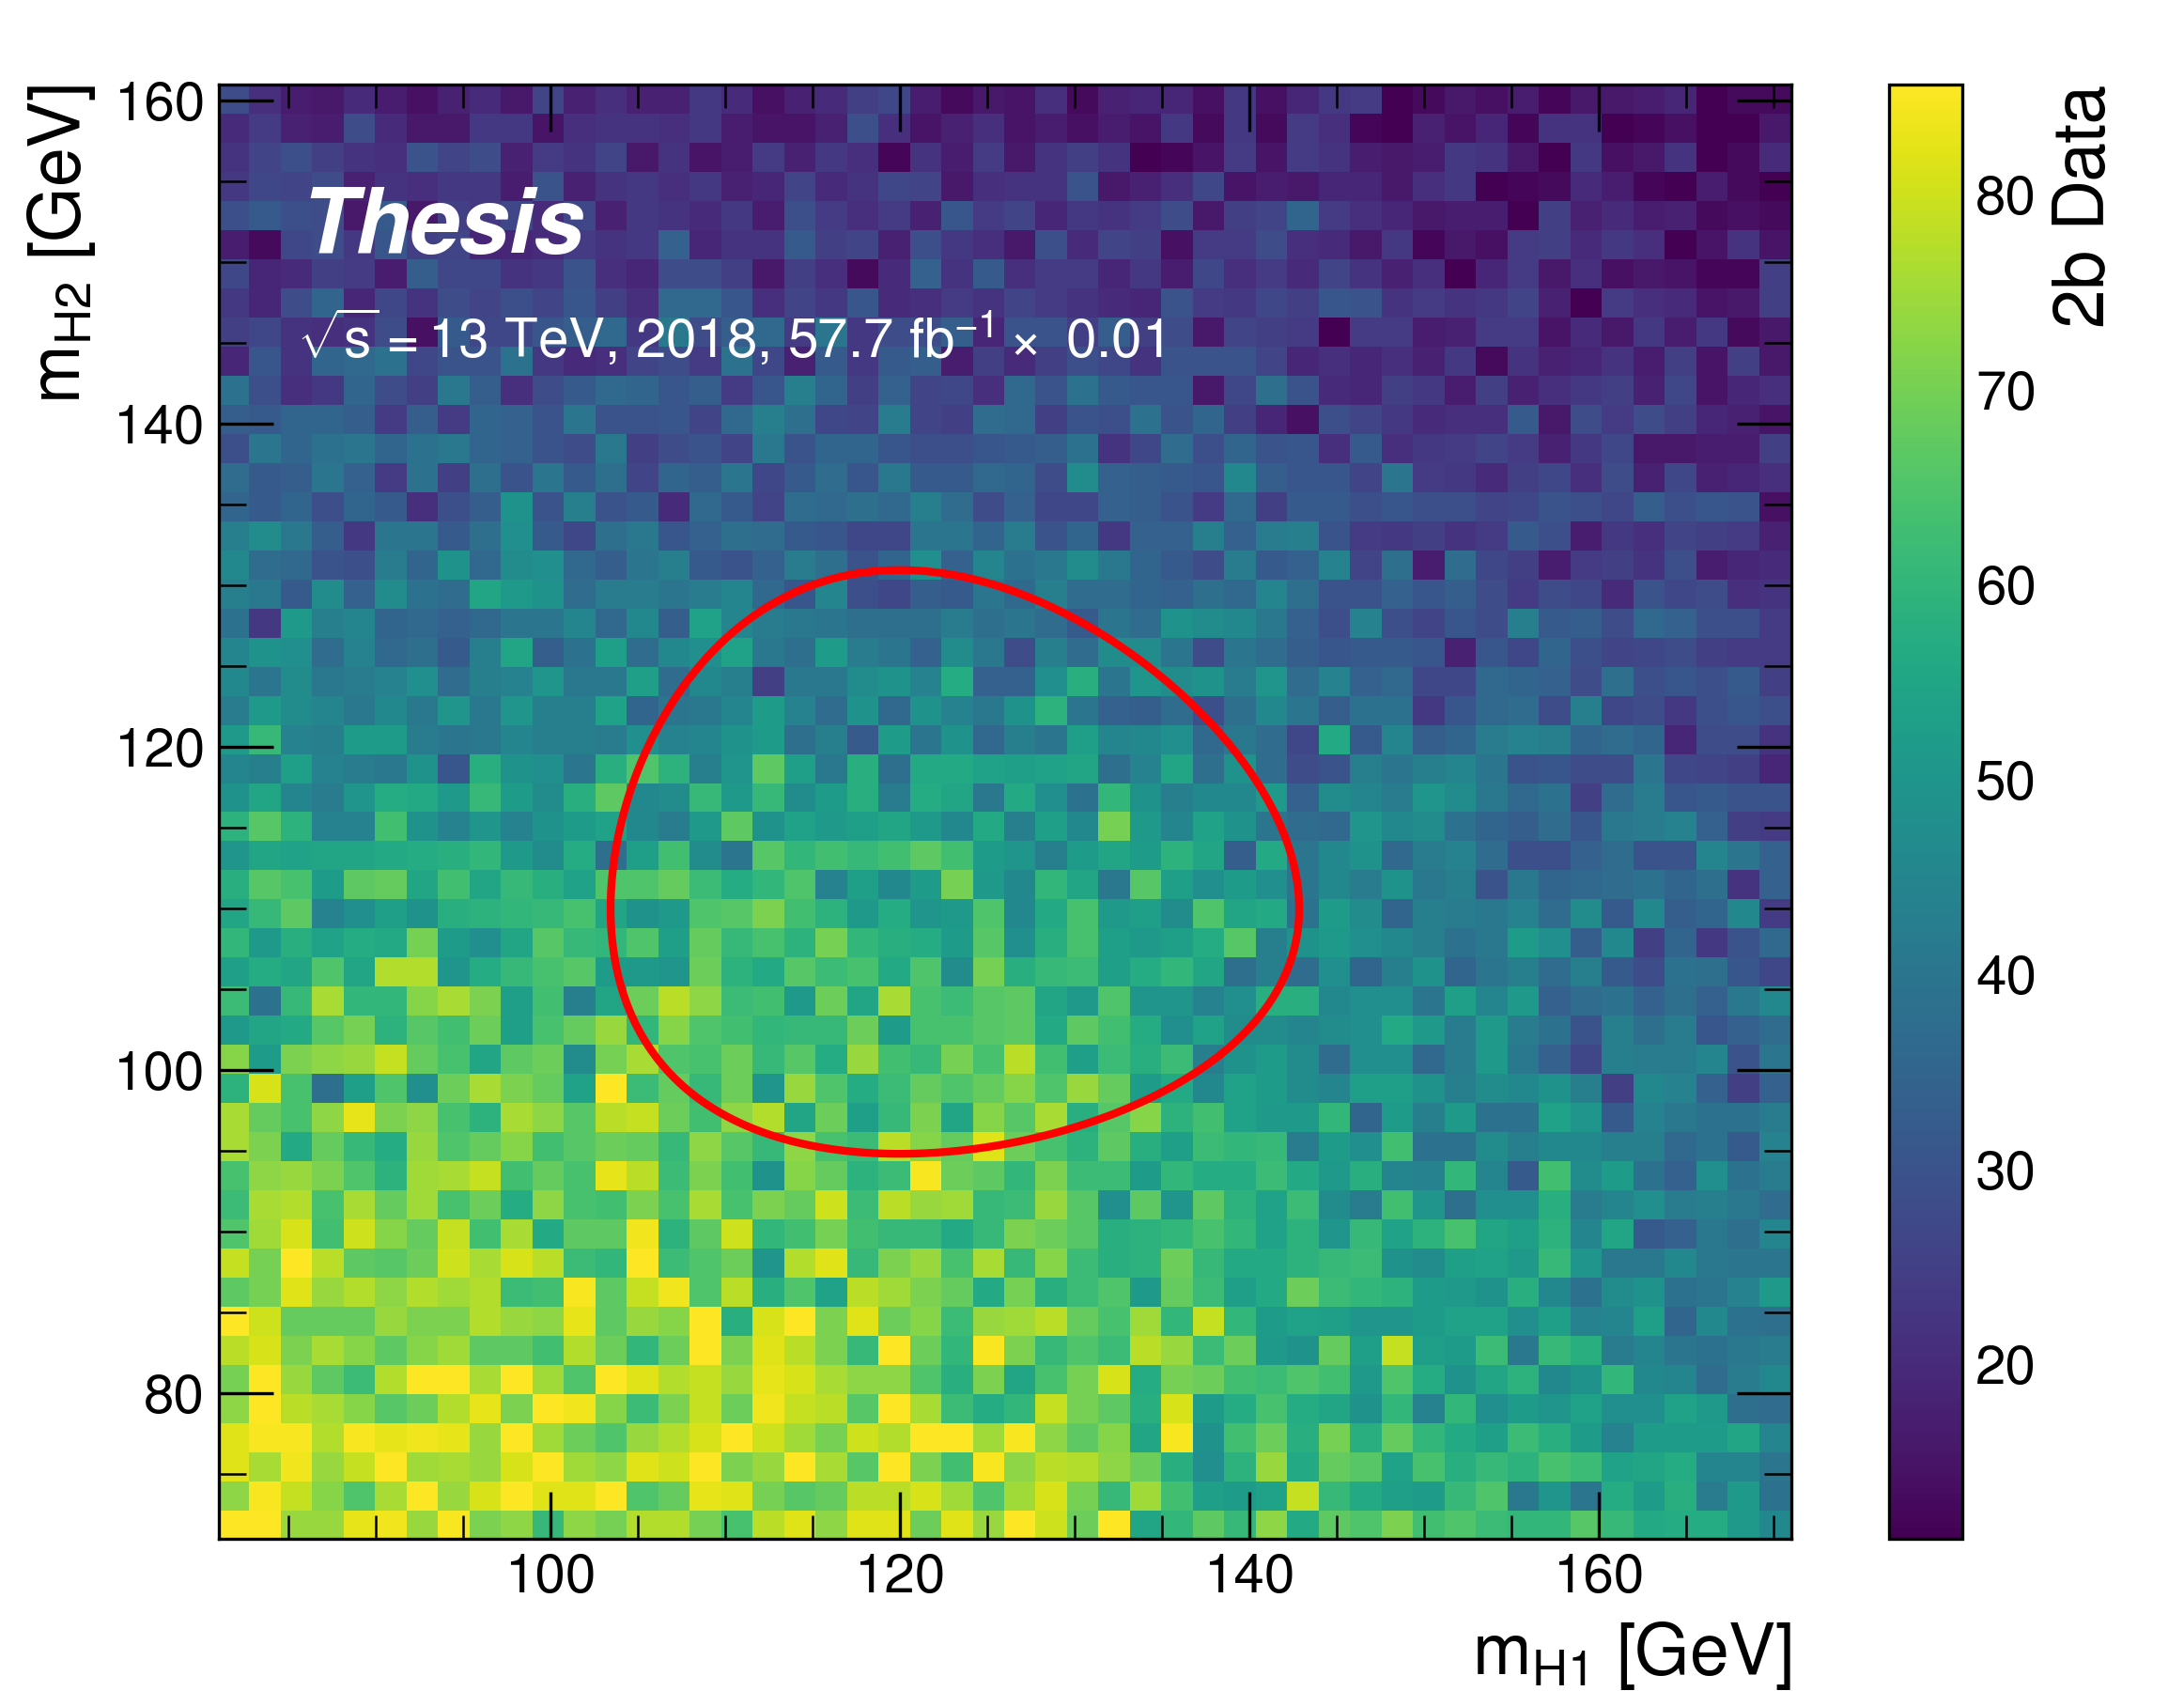
\includegraphics[width=0.48\textwidth]{figures/thesis-massplane-real-2b-0.01-2018-PAG.png}
	}
	\subfloat[Gaussian Process Sample]{\label{fig:gp-gen-18}%
		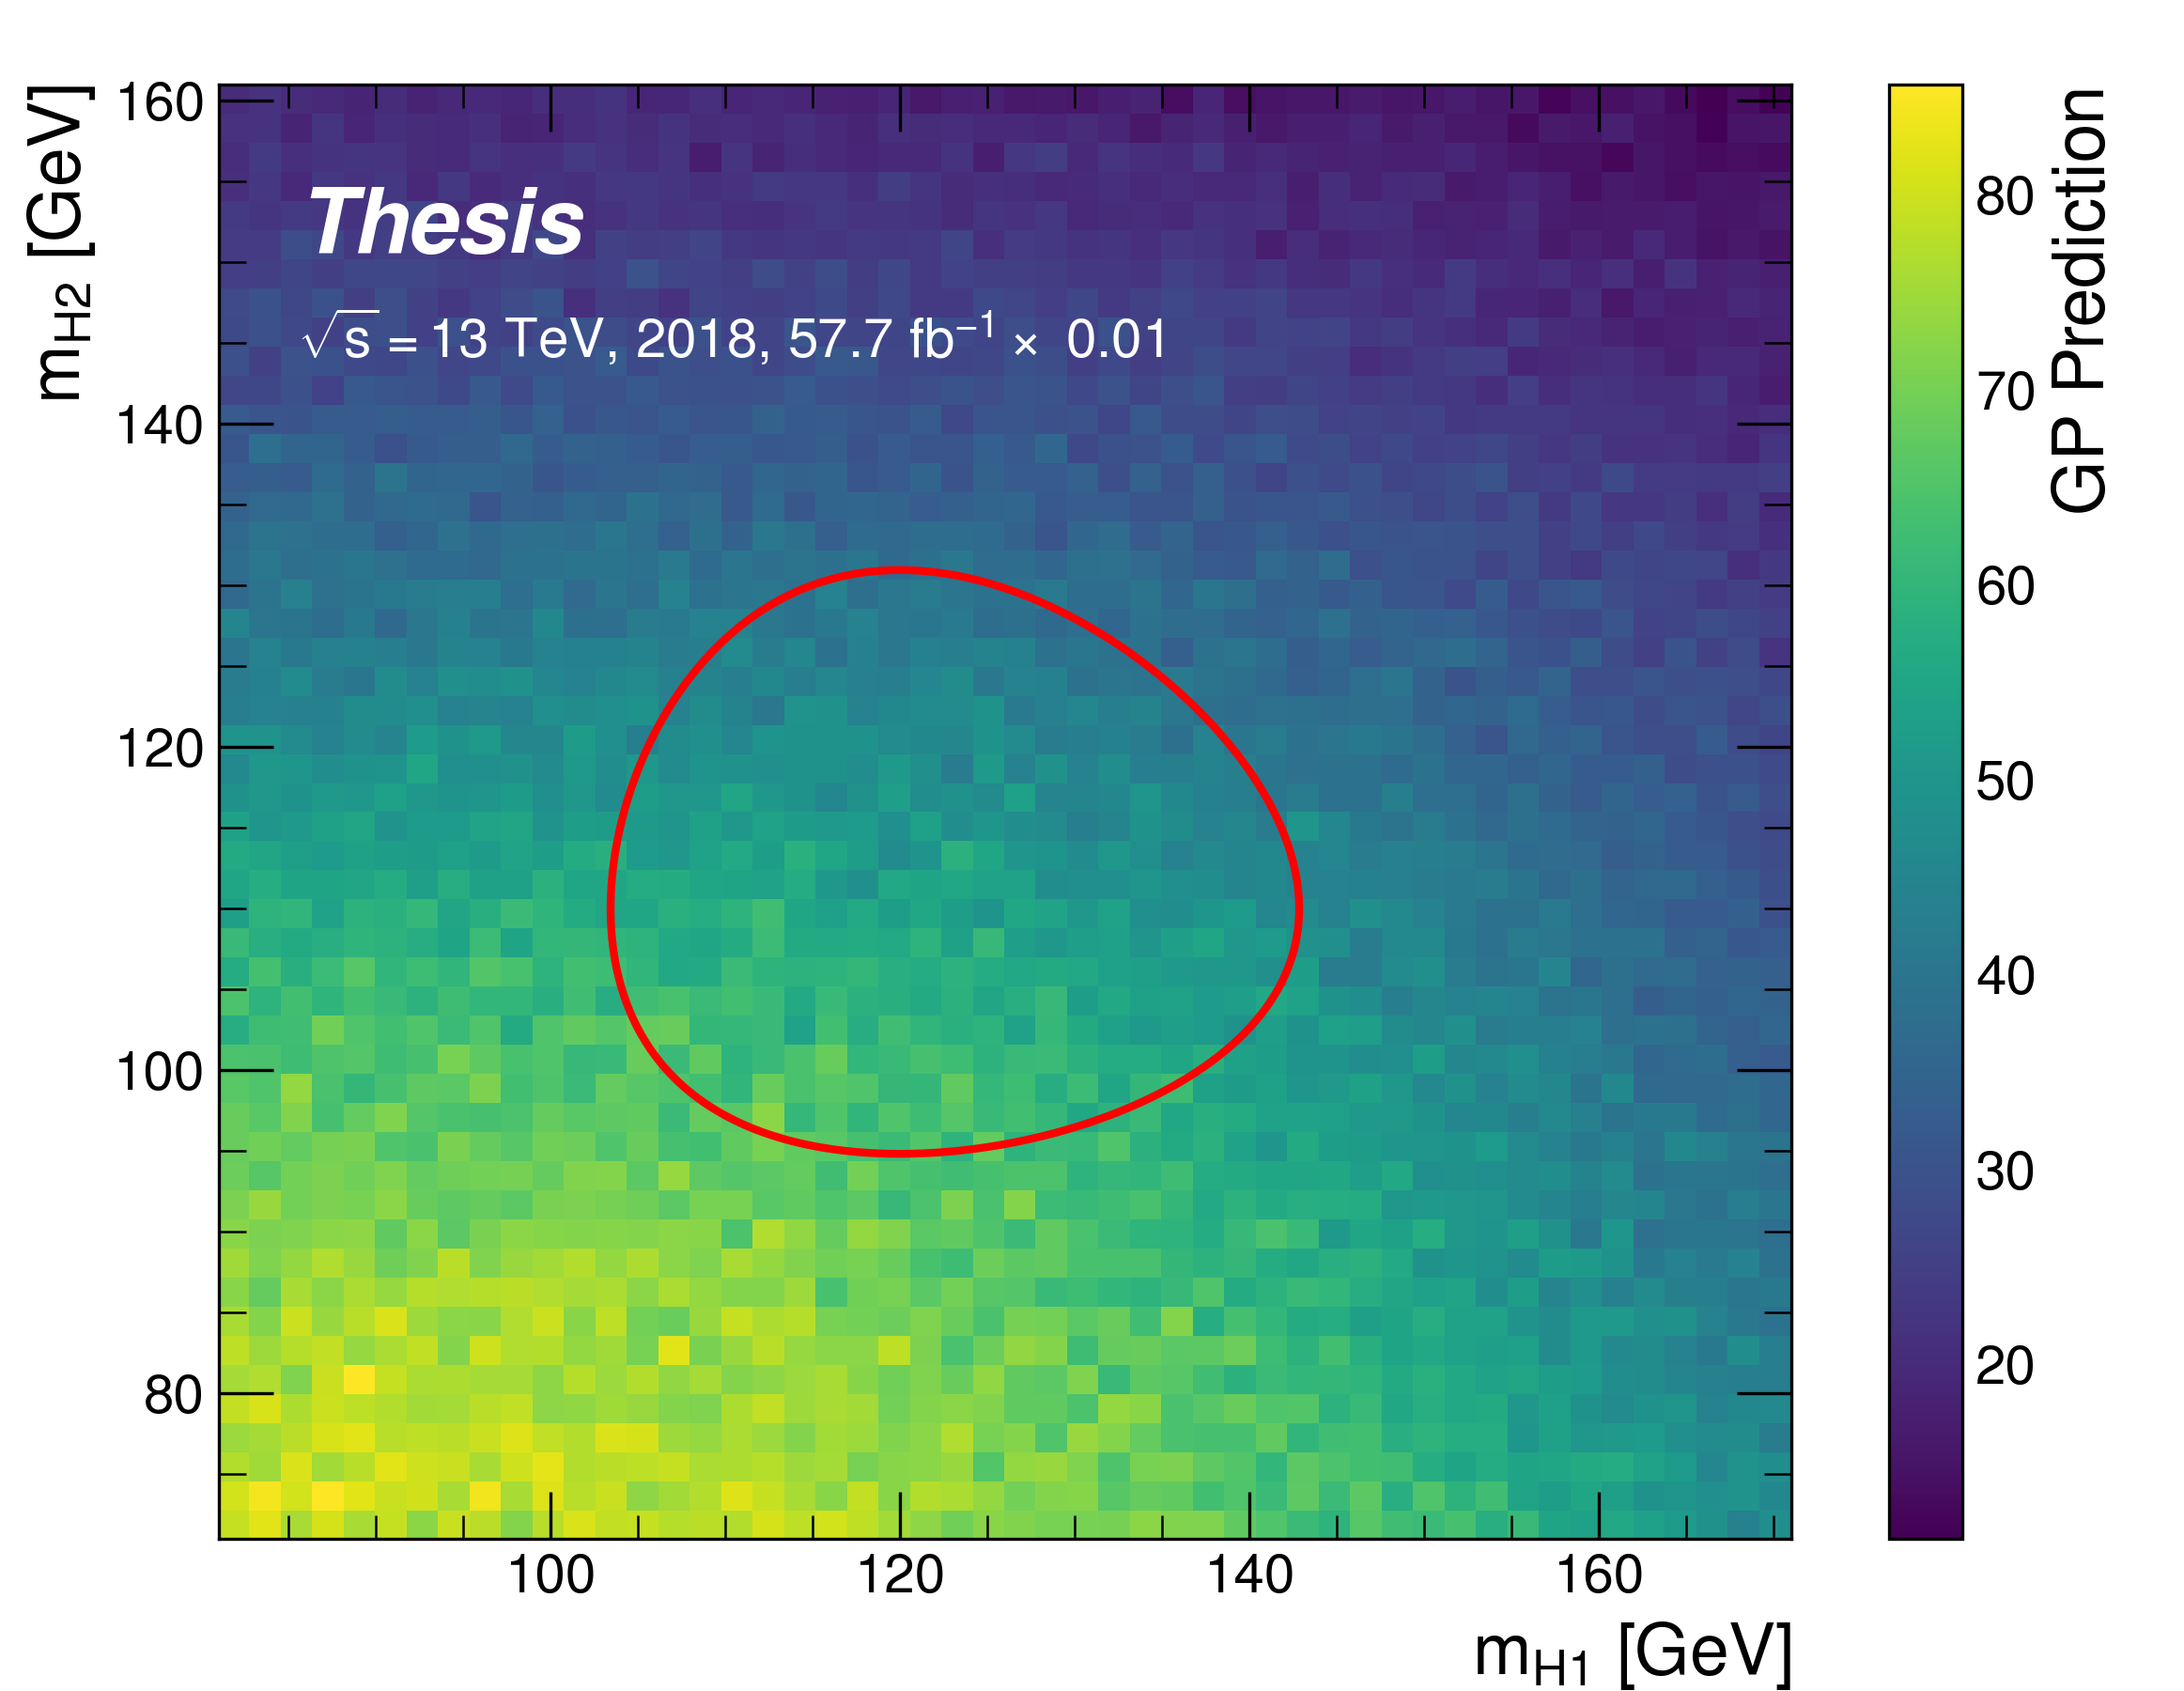
\includegraphics[width=0.48\textwidth]{figures/thesis-massplane-gen-2b-0.01-2018-PAG.png}
	}

	\subfloat[Ratio]{\label{fig:gp-ratio-18}%
		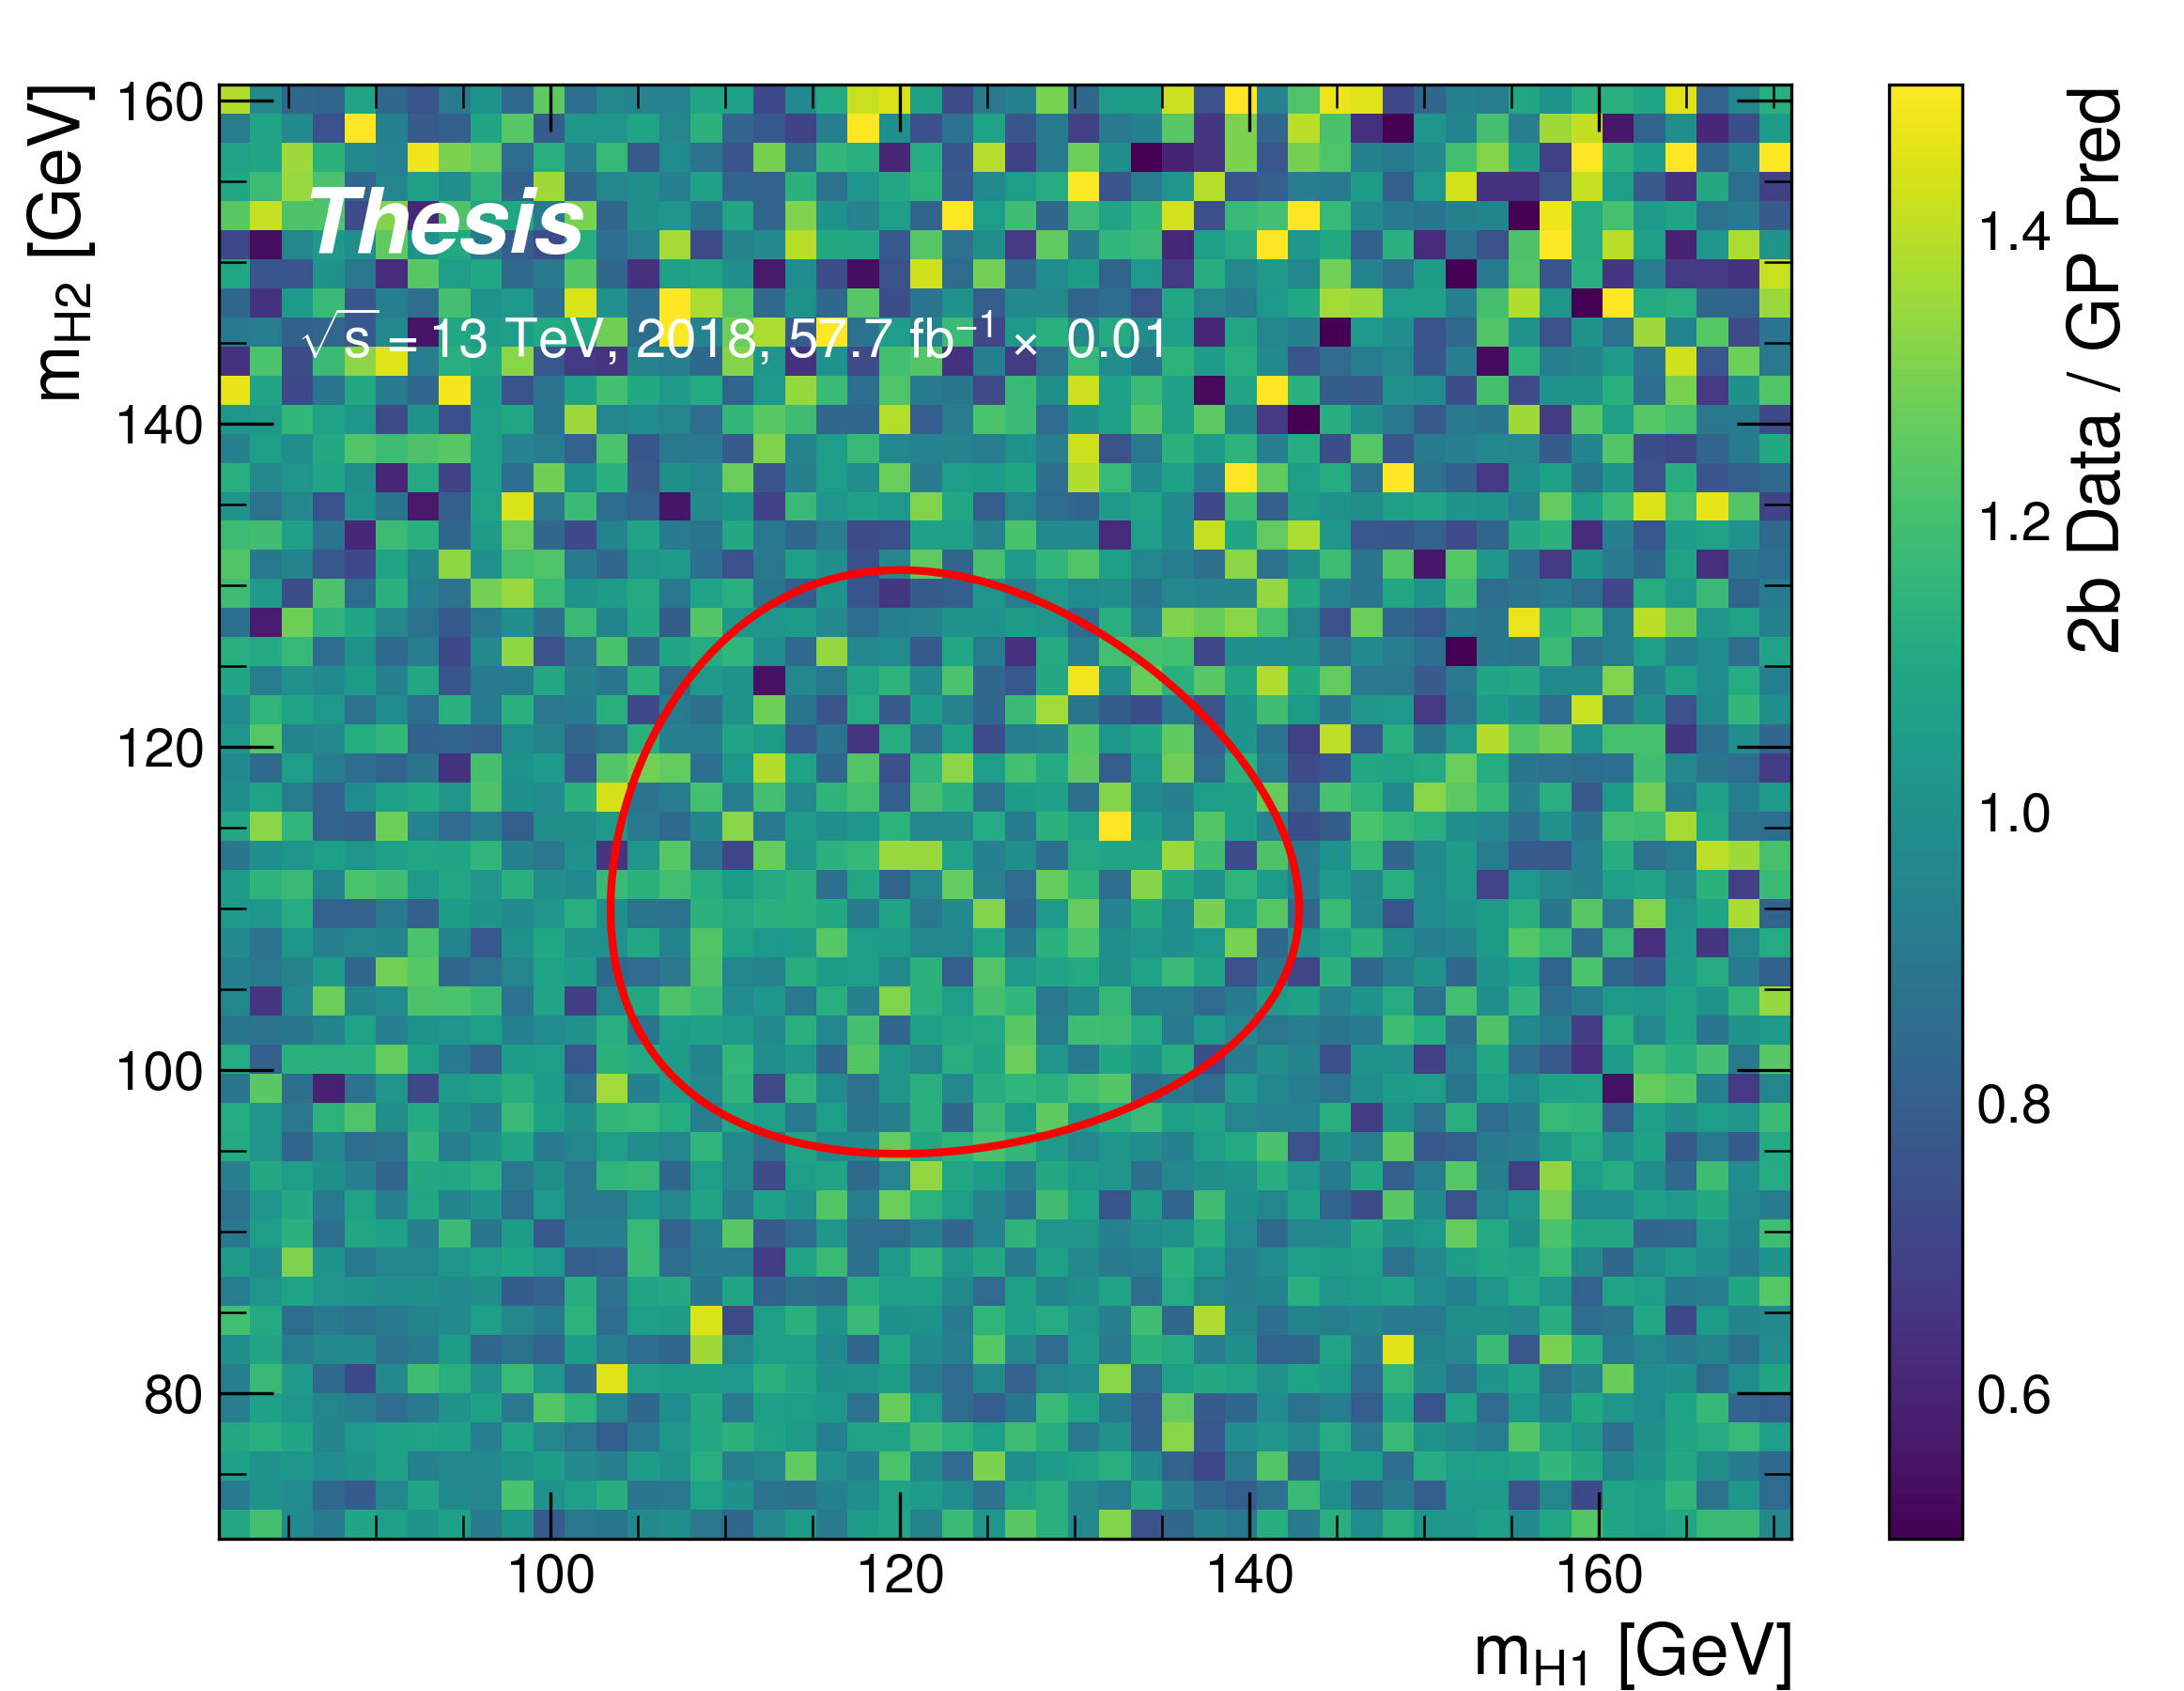
\includegraphics[width=0.48\textwidth]{figures/thesis-massplane-ratio-real-2b-gen-2b-0.01-2018-PAG.png}
	}
	\caption{\label{fig:gp-massplane-18} Gaussian process sampling prediction for the mass plane compared to the real 
	$2b$ dataset for 2018. Only a small fraction ($0.01$) of the $2b$ dataset is used for both training and this final 
	comparison to mimic $4b$ statistics. Good agreement is seen.}
\end{figure}

The $4b$ region is kept blinded for this work, meaning that a direct comparison of the Gaussian process 
estimate in the $4b$ signal region is not done. However, a Gaussian process is trained on the blinded $4b$ 
region and compared to the corresponding reweighted $2b$ estimate, trained per the nominal procedures from
the analyses above. The predictions for signal region $m_{H1}$ and $m_{H2}$ individually are shown in 
Figure \ref{fig:gp-marginals-4b-18}, compared to both the control and validation region derived reweighting estimates,
and the resulting signal region mass planes are compared in Figure \ref{fig:gp-massplane-4b-18}. The 
estimates are seen to be compatible.

\begin{figure}[ht]
	\centering
	\subfloat{\label{fig:gp-4b-mh1-18}%
		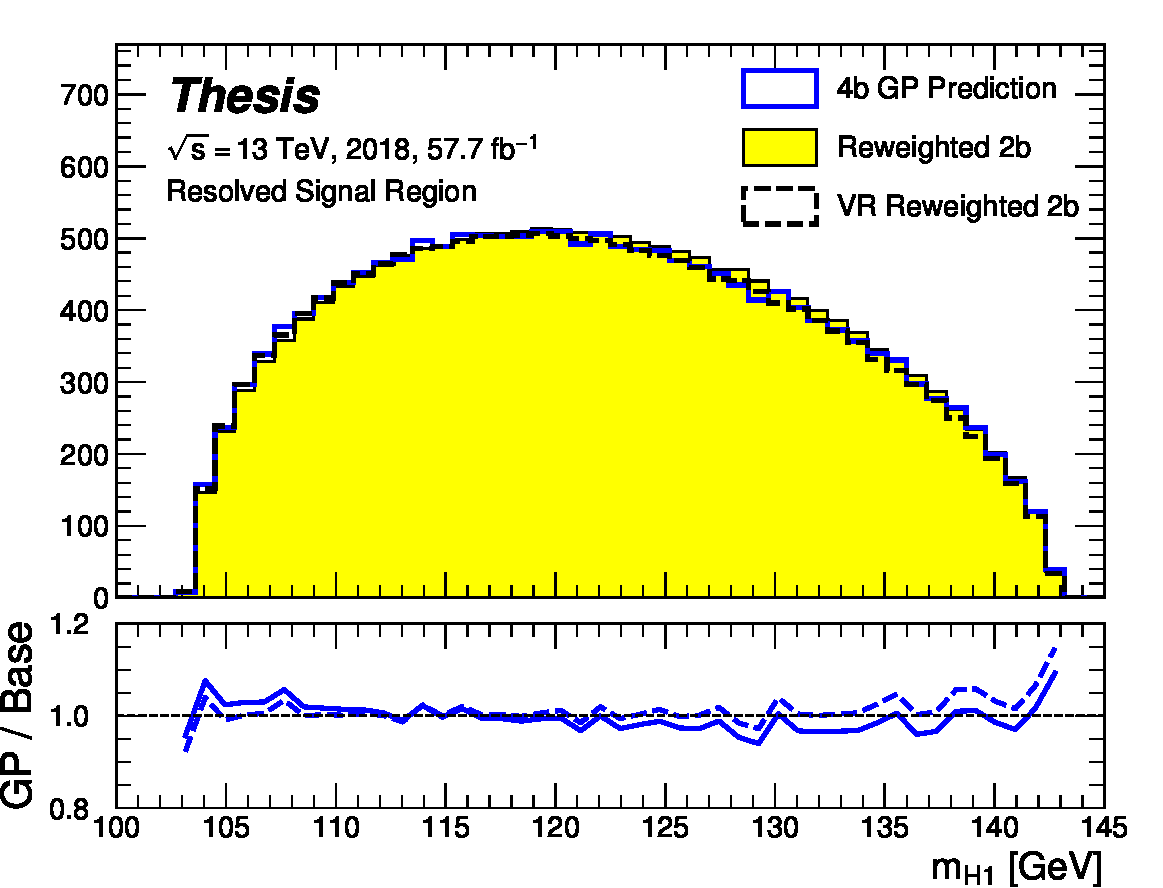
\includegraphics[width=0.48\textwidth]{figures/thesis-pure4b-GP-vs-rw2b-withVR-2018-Signal-m-h1.pdf}
	}
	\subfloat{\label{fig:gp-4b-mh2-18}%
		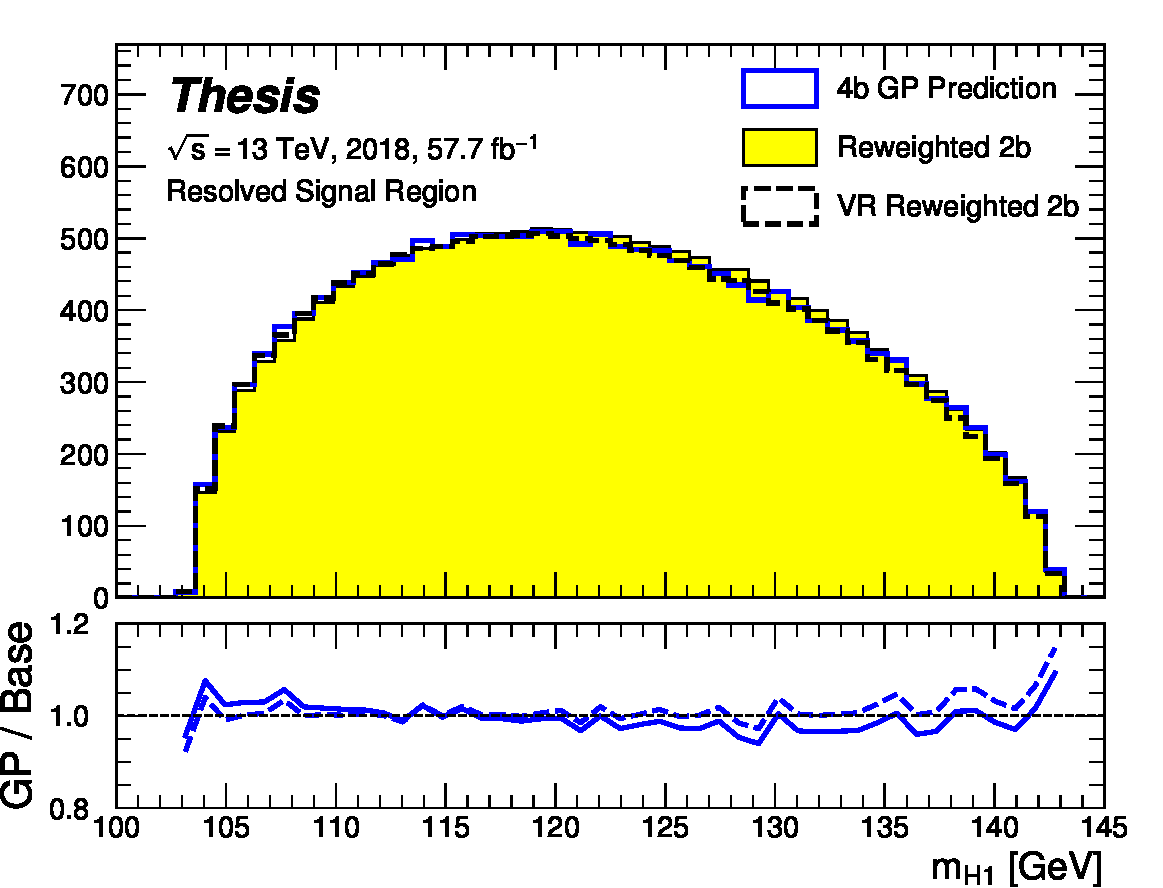
\includegraphics[width=0.48\textwidth]{figures/thesis-pure4b-GP-vs-rw2b-withVR-2018-Signal-m-h1.pdf}
	}
	\caption{\label{fig:gp-marginals-4b-18} Gaussian process sampling prediction of marginals $m_{H1}$ and $m_{H2}$ 
	for $4b$ signal region events compared to both control and validation reweighting predictions. While there
	are some differences, the estimates are compatible.}
\end{figure}


\begin{figure}[ht]
	\centering
	\subfloat[Reweighted 2b Data]{\label{fig:gp-rw2b-18}%
		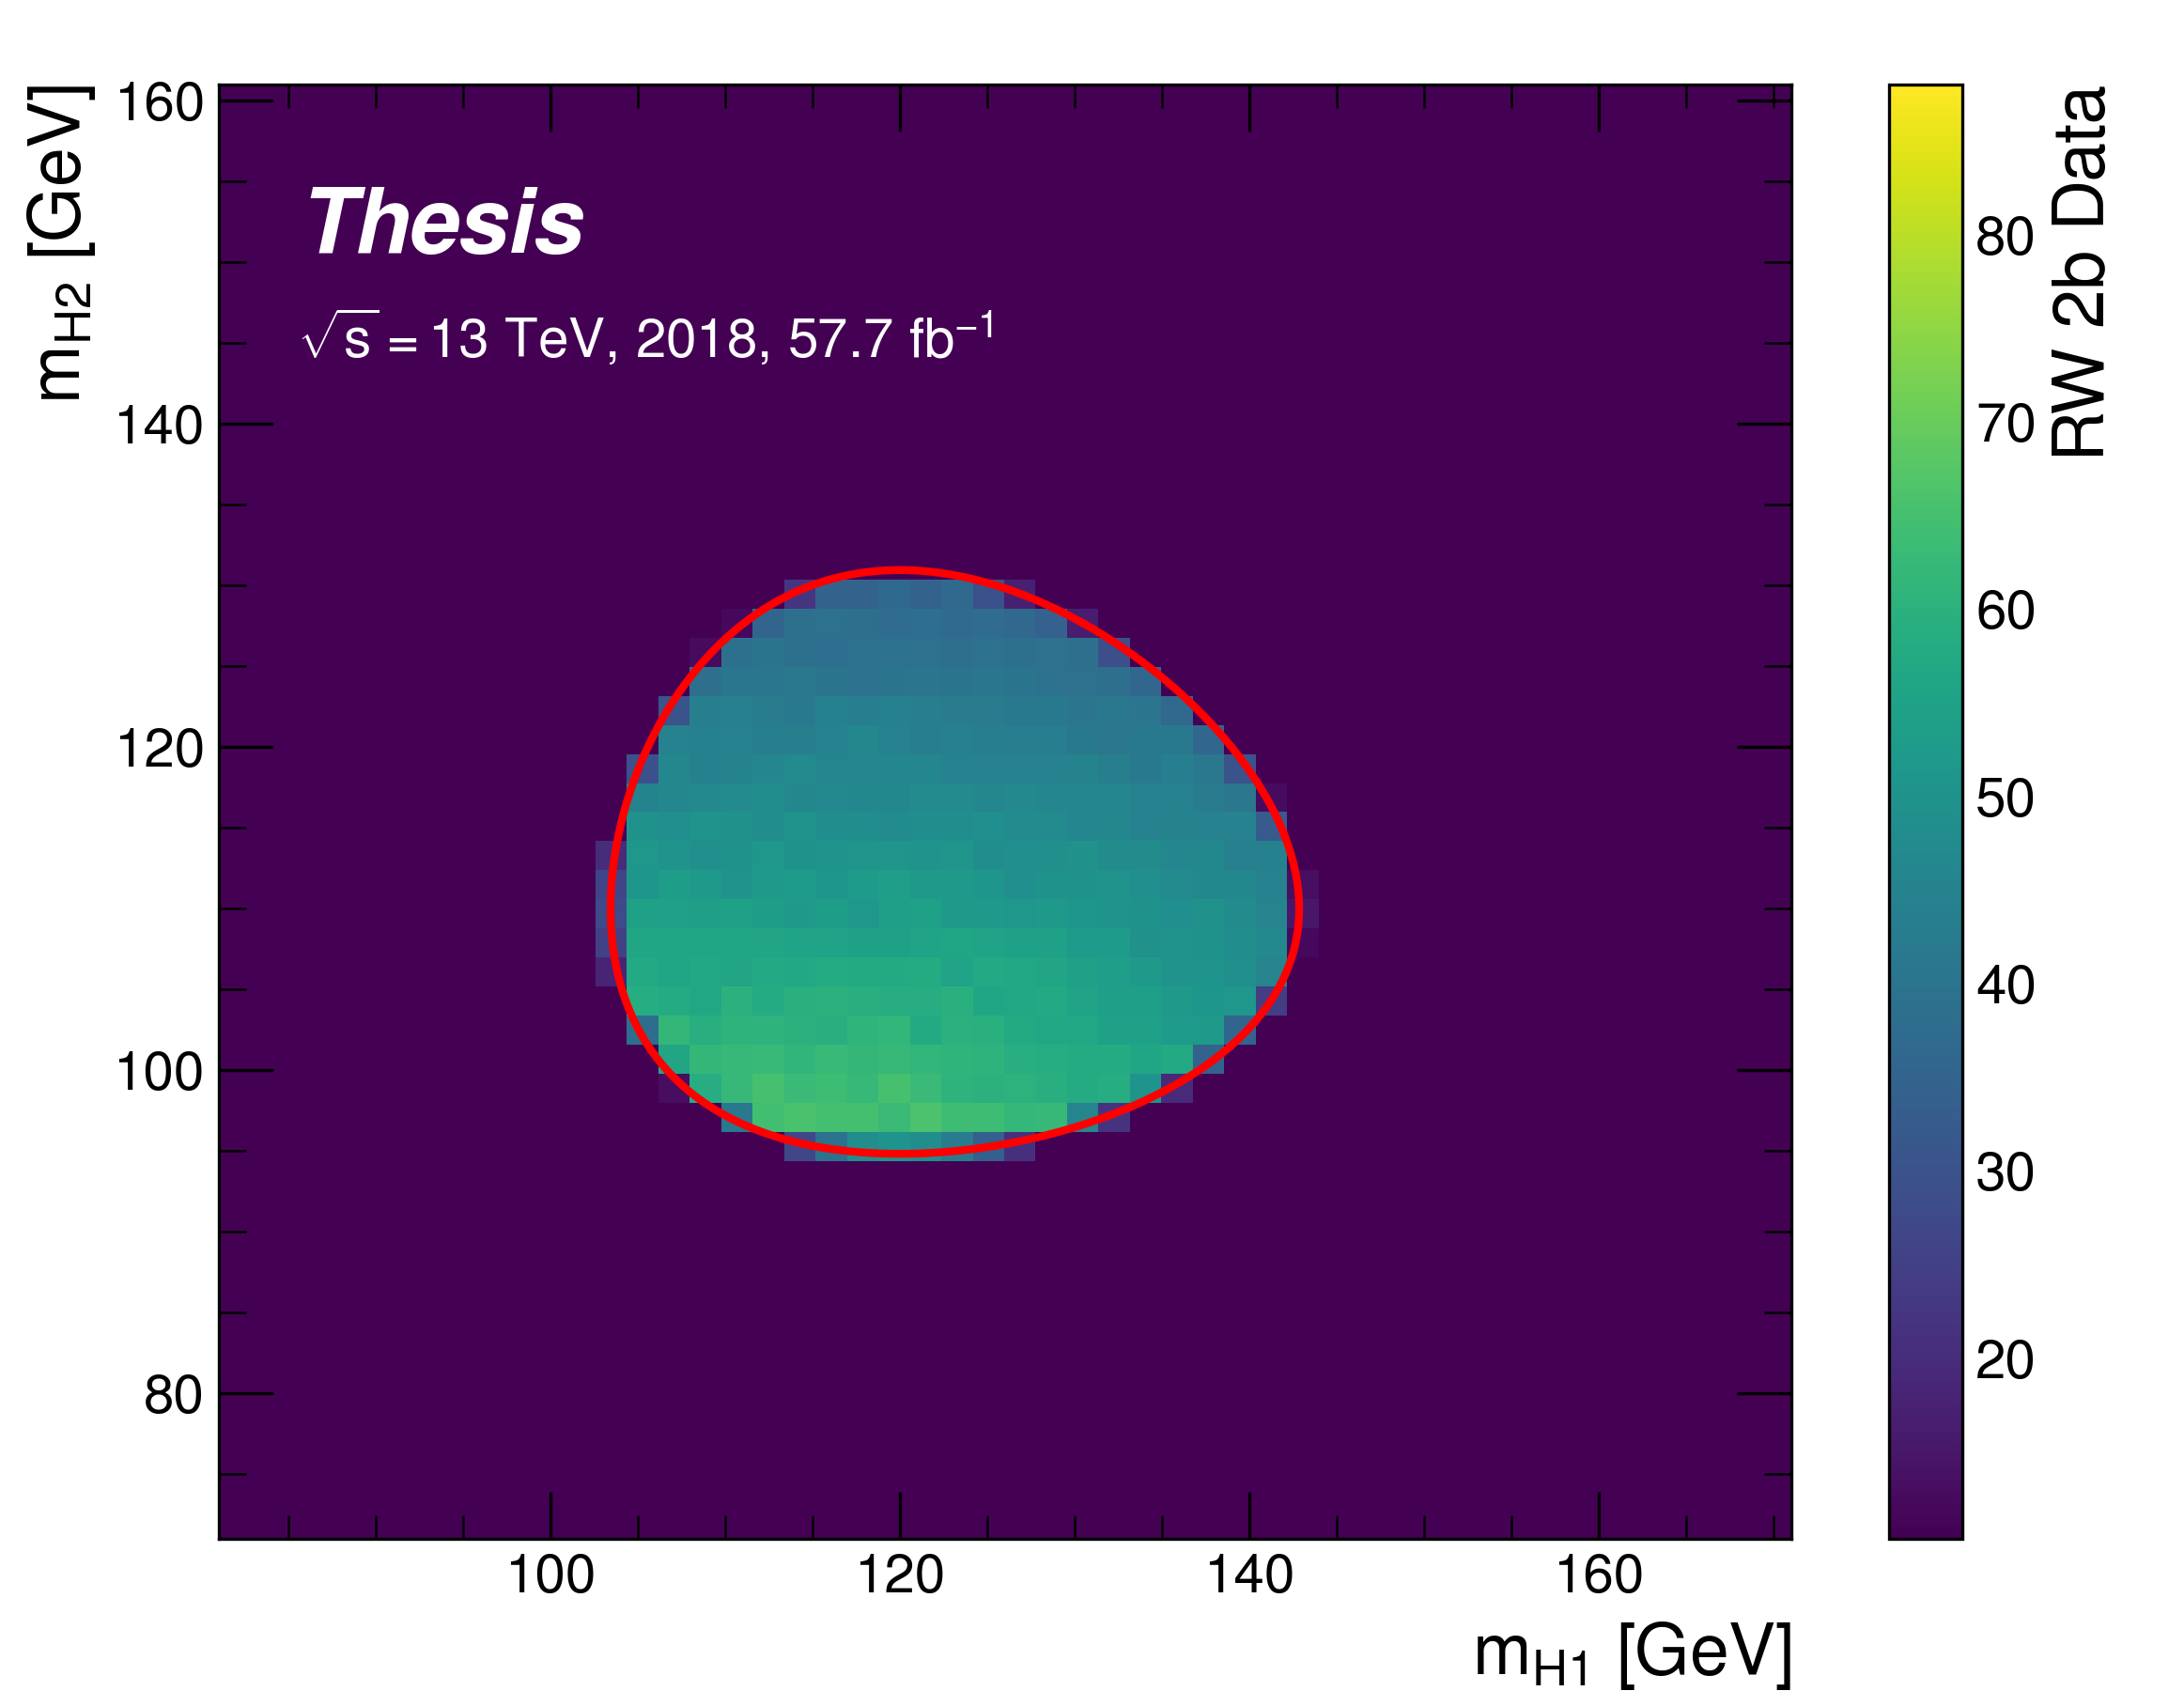
\includegraphics[width=0.48\textwidth]{figures/massplane-rw-2b-2018-PAG.png}
	}
	\subfloat[Gaussian Process Sample]{\label{fig:gp-gen-4b-18}%
		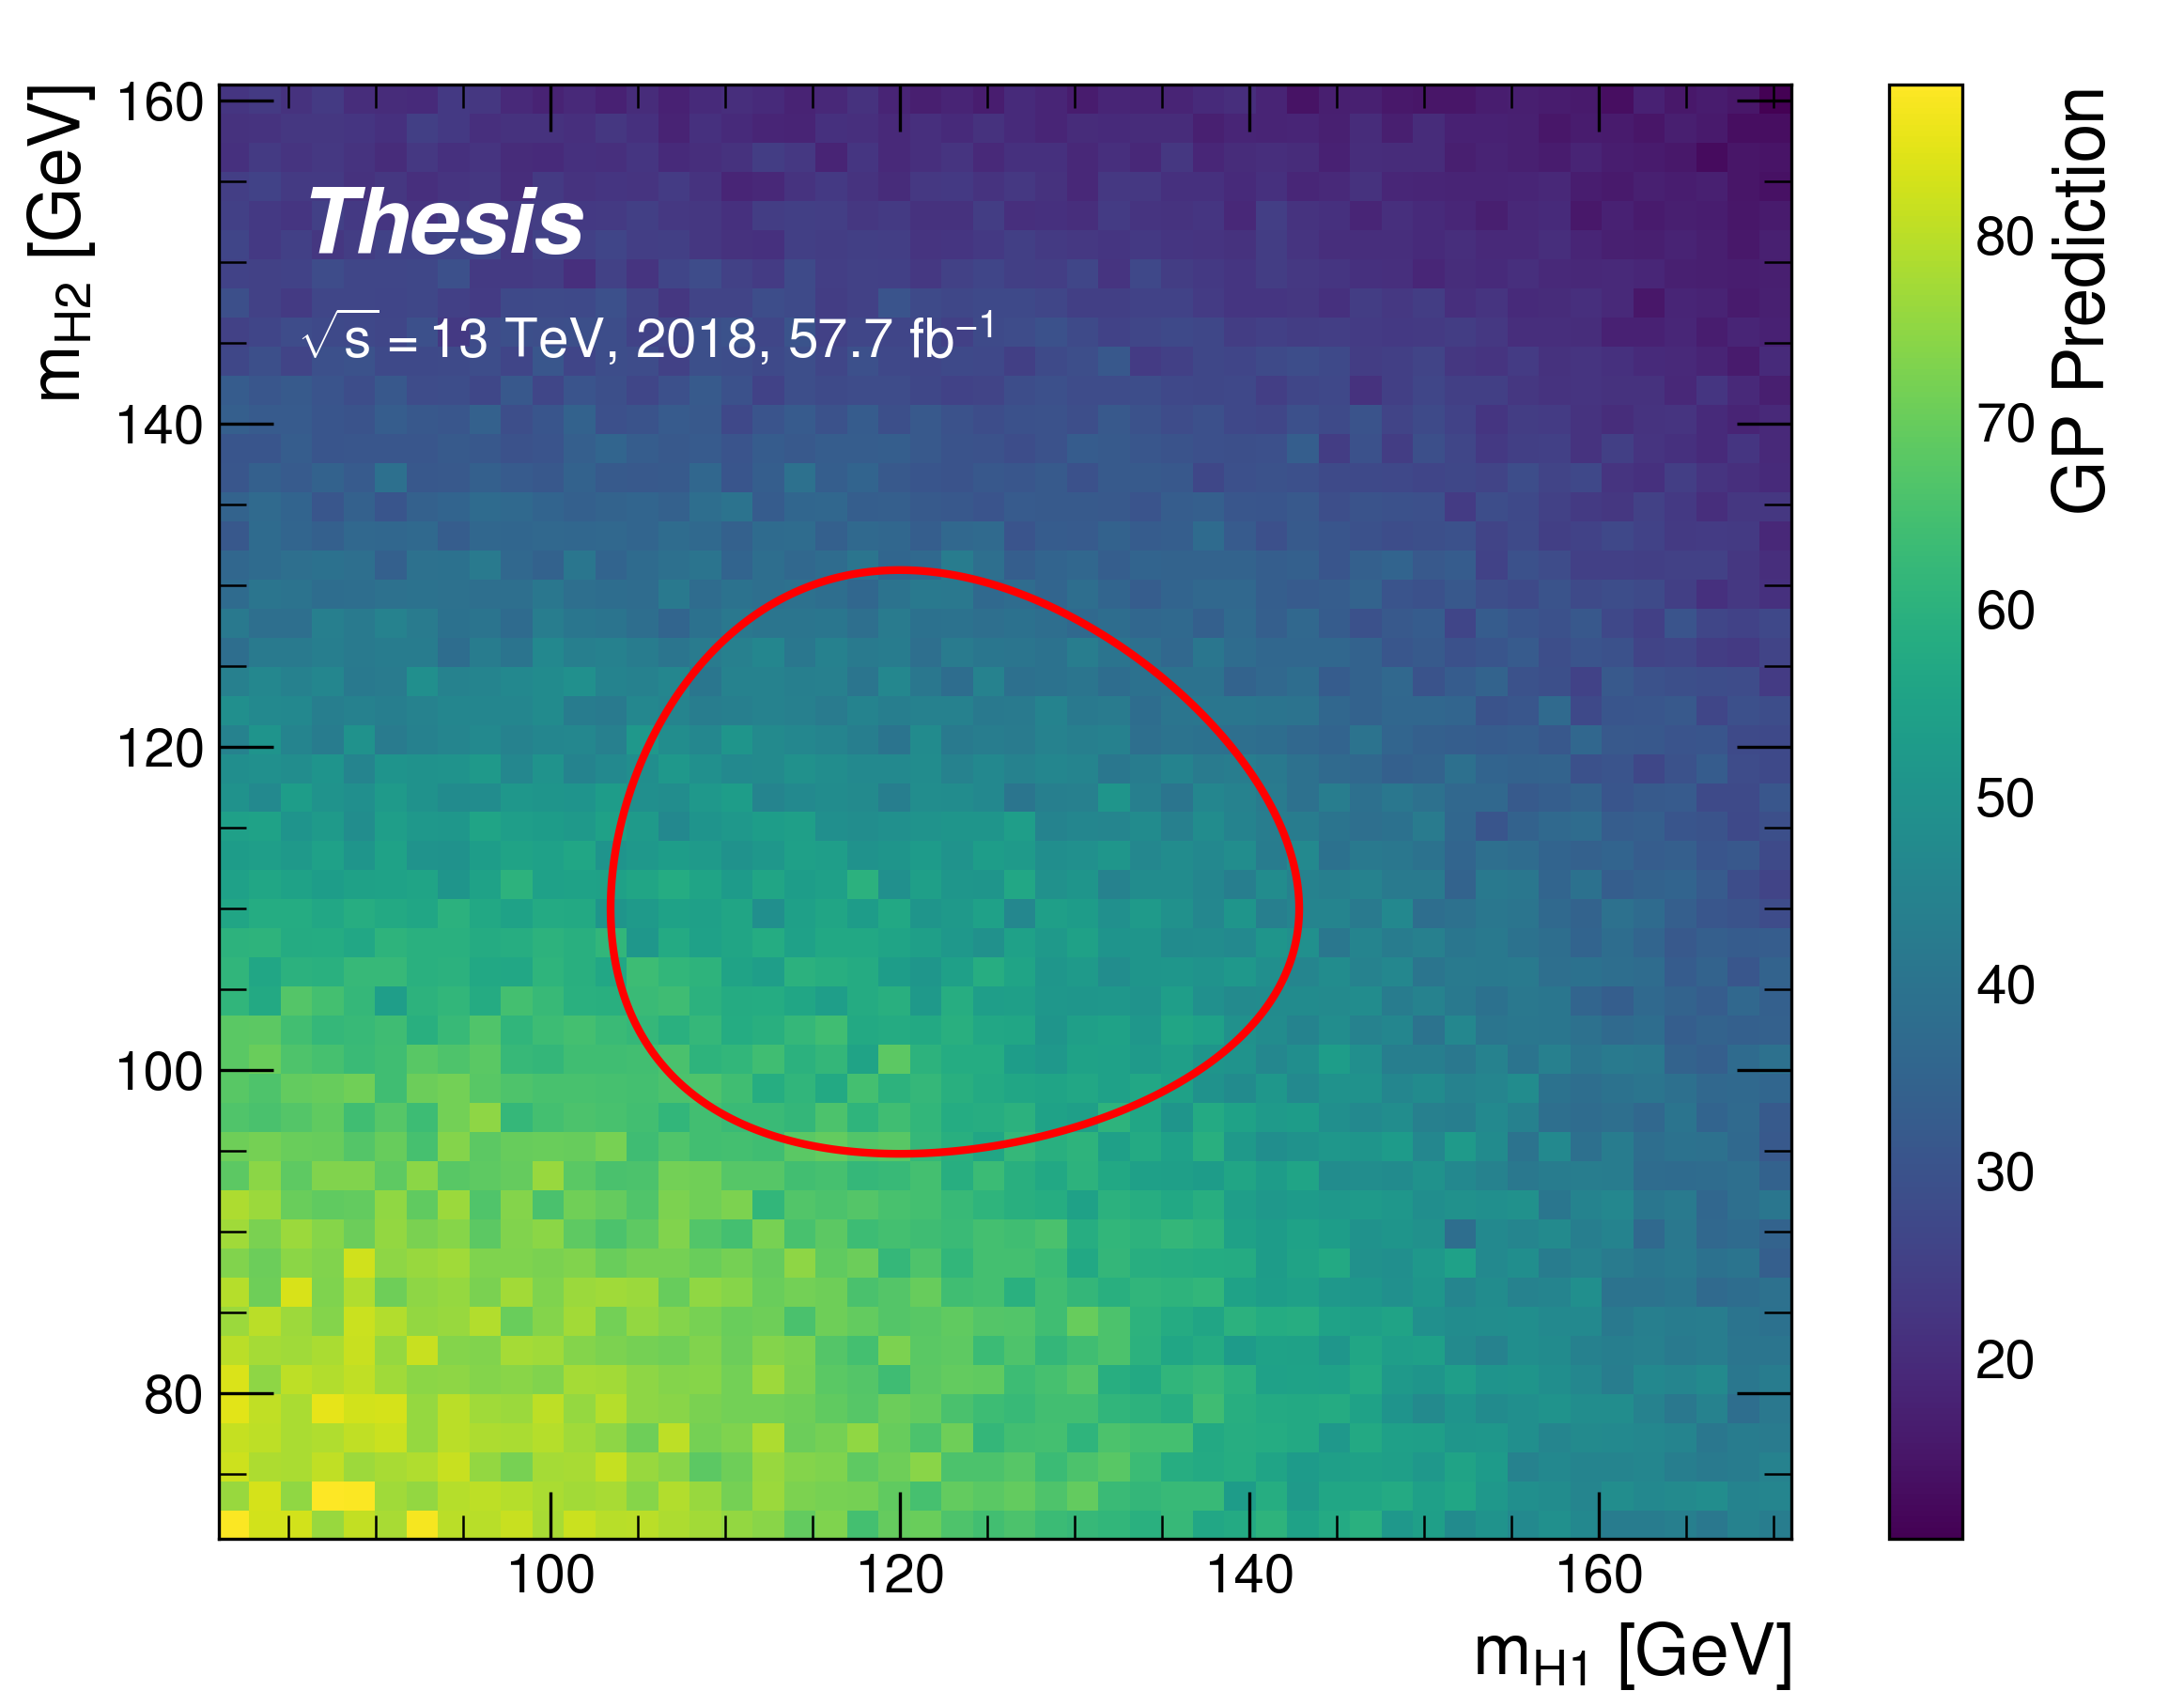
\includegraphics[width=0.48\textwidth]{figures/thesis-massplane-gen-4b-2018-PAG.png}
	}

	\subfloat[Ratio]{\label{fig:gp-ratio-4b-rw-2b-18}%
		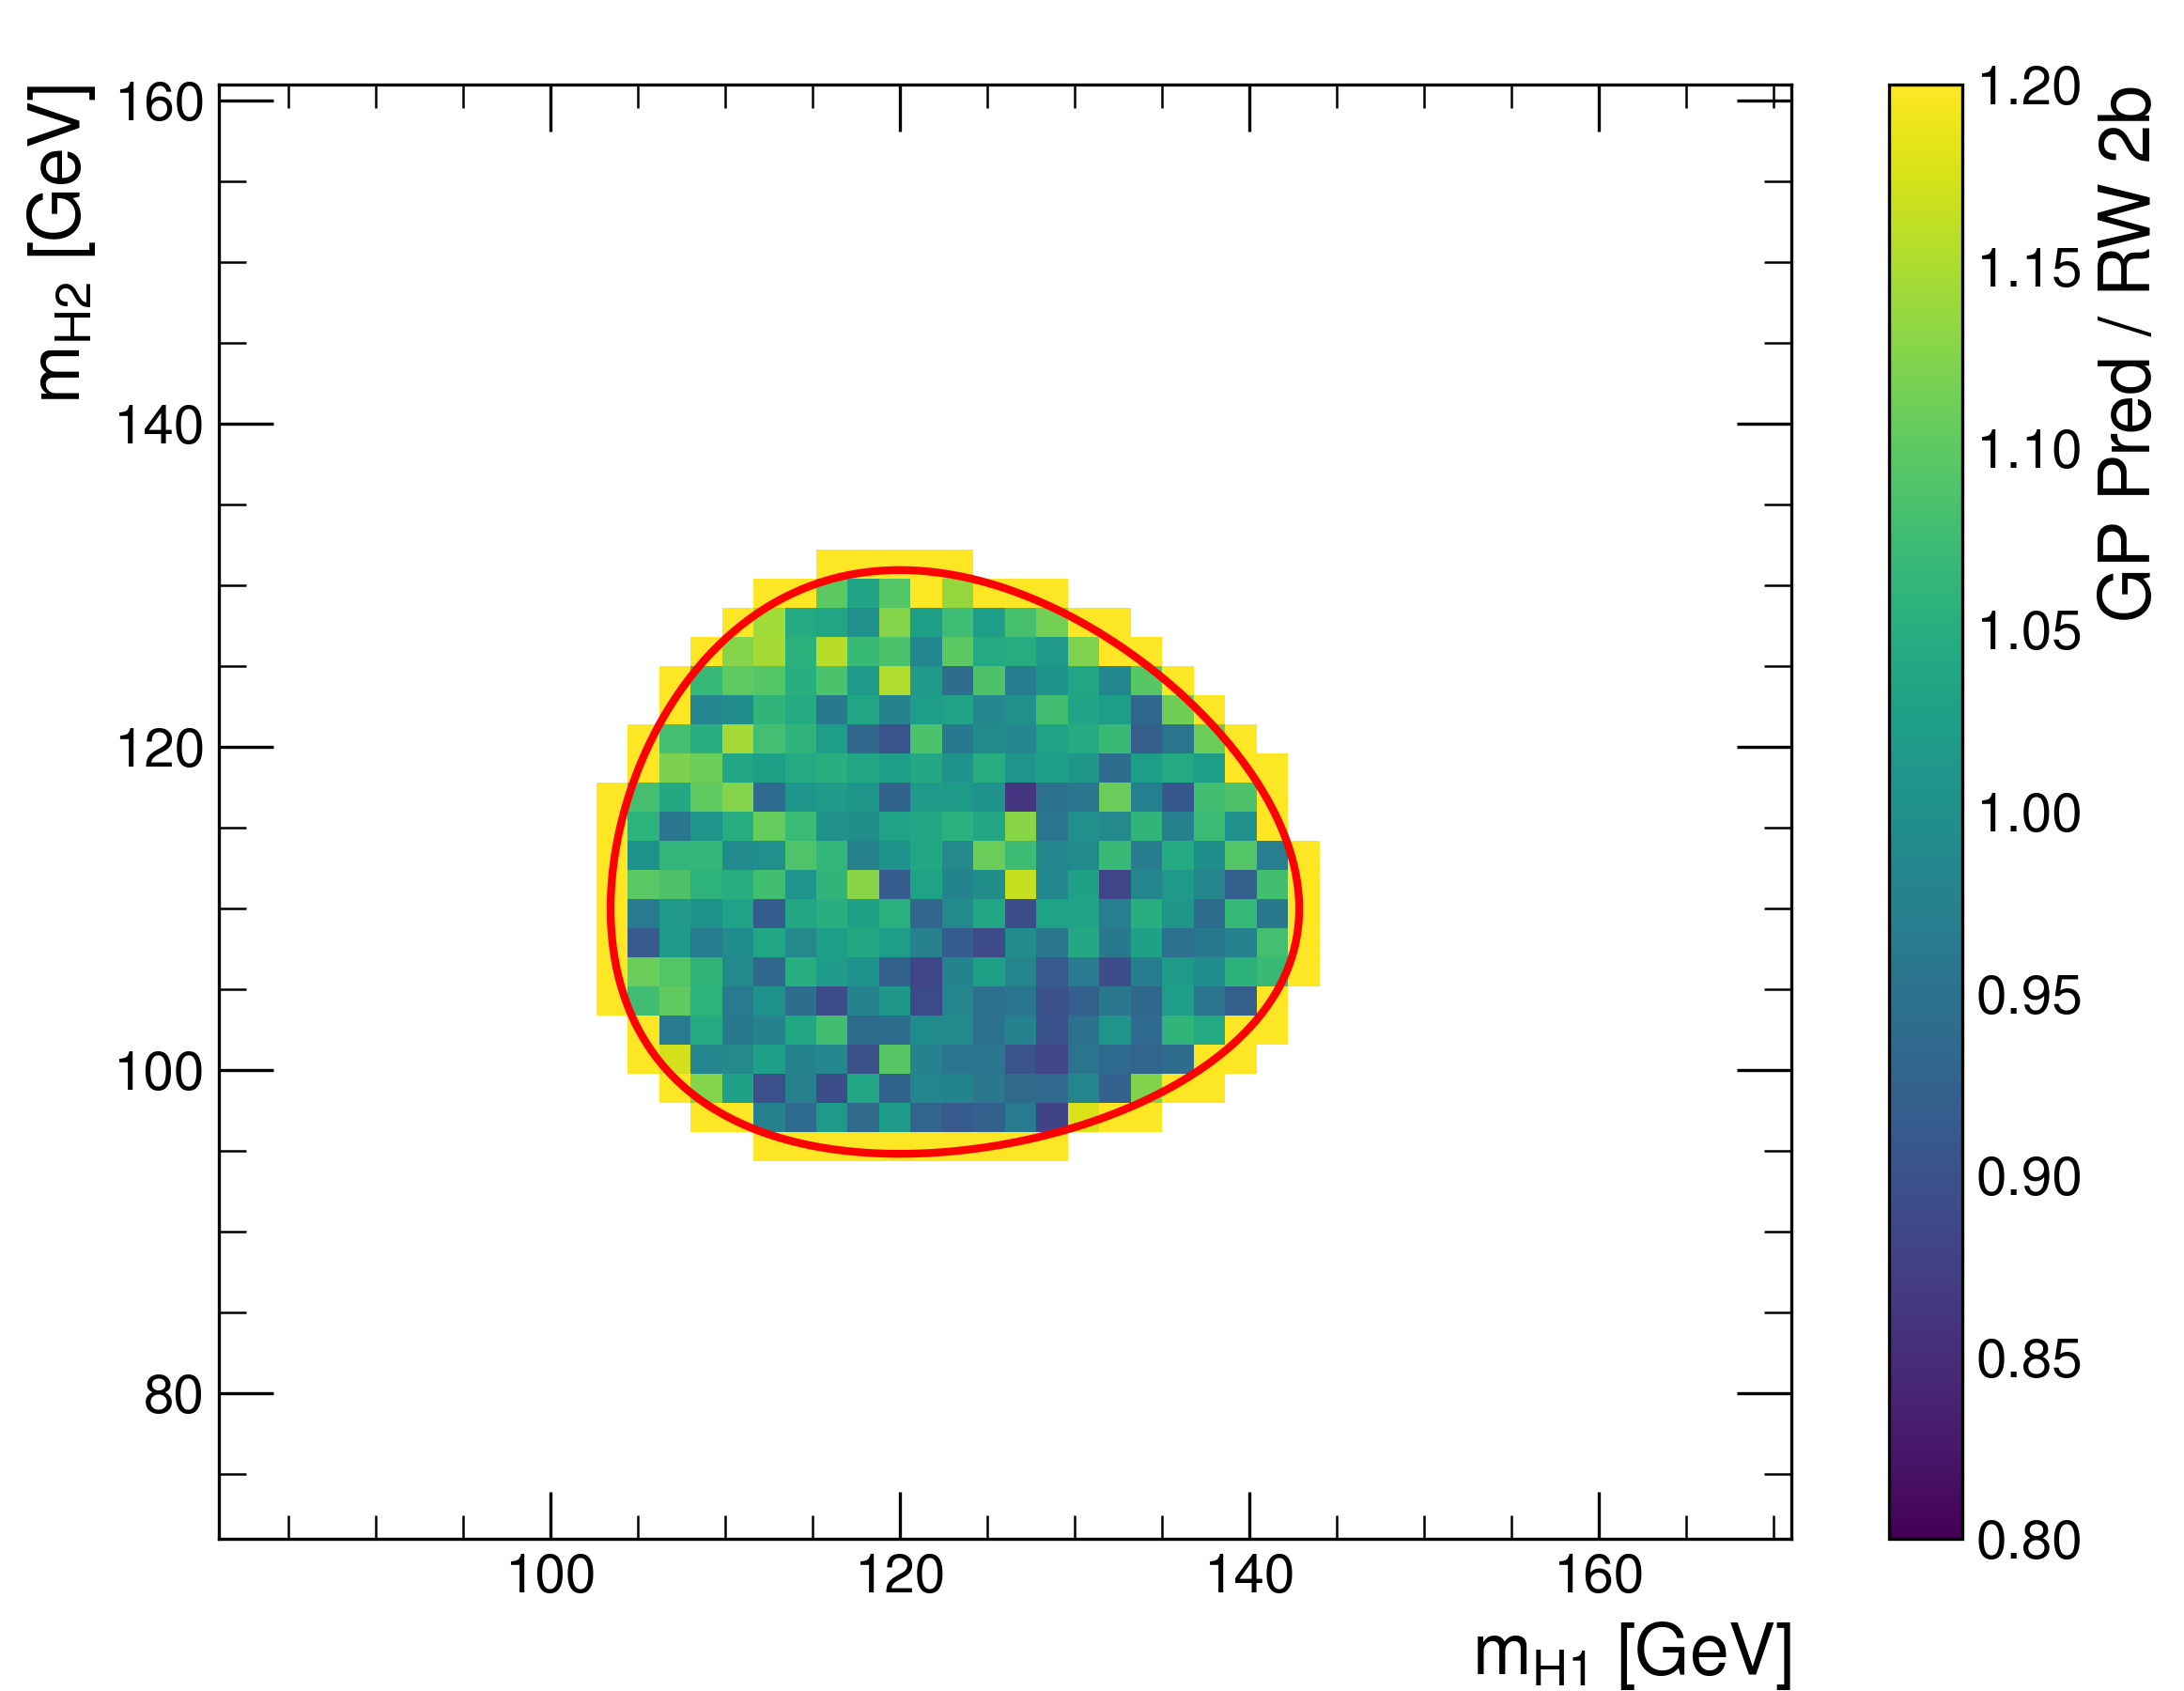
\includegraphics[width=0.48\textwidth]{figures/thesis-massplane-ratio-gen-4b-rw-2b-2018-PAG.png}
	}
	\caption{\label{fig:gp-massplane-4b-18} Gaussian process sampling prediction for the $4b$ mass plane compared to 
	the reweighted $2b$ estimate in the signal region. Both estimates are compatible.}
\end{figure}

The Gaussian process estimate may then be used as an input to the normalizing flow estimate to form a 
complete background estimate. Figure \ref{fig:flow-gp-2b} shows such an estimate for the subsampled $2b$ 
signal region. Results for the prediction of the normalizing flow with 
inputs of real 2b signal region $m_{H1}$ and $m_{H2}$ are compared to the results of using Gaussian 
process predicted $m_{H1}$ and $m_{H2}$, and are seen to be consistent, demonstrating the above 
closure of the Gaussian process prediction. Reasonable agreement with real $2b$ signal region 
data is seen.

\begin{figure}
\centering
	\subfloat{
	    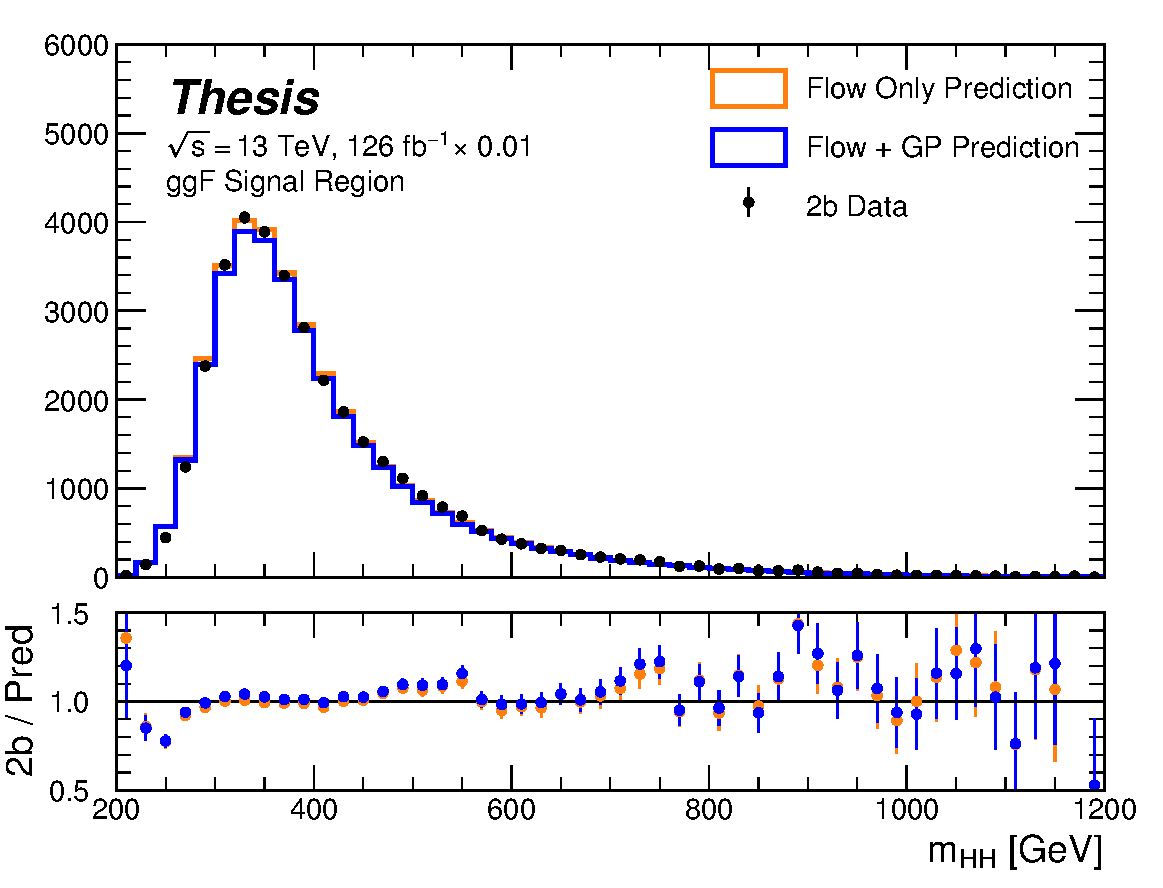
\includegraphics[width=0.8\textwidth]{figures/m-hh-comparison-flow-gp-2b.pdf}
	}
	\caption{\label{fig:flow-gp-2b} Comparison of the interpolation background estimate with 
	real 2b data in the signal region. Only 1~\% of $2b$ data is used in order to mimic $4b$ statistics, 
	and results are presented here summed across years. The ``Flow Only'' prediction uses samples of 
	actual $2b$ signal region data for the input values of $m_{H1}$ and $m_{H2}$, whereas the ``Flow + GP'' 
	prediction uses samples following the Gaussian process procedure above, more closely mimicking a 
	the full background estimation procedure. The two predictions are quite comparable, demonstrating the 
	closure of the Gaussian process estimate, and the predicted $m_{HH}$ shape agrees well with $2b$ data. 
	Only $2b$ statistical uncertainty is shown.}
\end{figure}


Figure \ref{fig:flow-gp-rw-4b} demonstrates the application of this process to the $4b$ region, 
closely following how such an estimate would be used in the $HH\rightarrow\bbbb$ analysis. As the 
$4b$ signal region is kept blinded for these studies, no direct evaluation is made, but results 
are compared to a resonant control region derived reweighting. Both signal region predictions are 
seen to be comparable, though there are some systematic differences. However, only the nominal 
estimates are compared here, with assessment of uncertainties on the interpolated estimate 
left for future work.

\begin{figure}
\centering
	\subfloat{
	    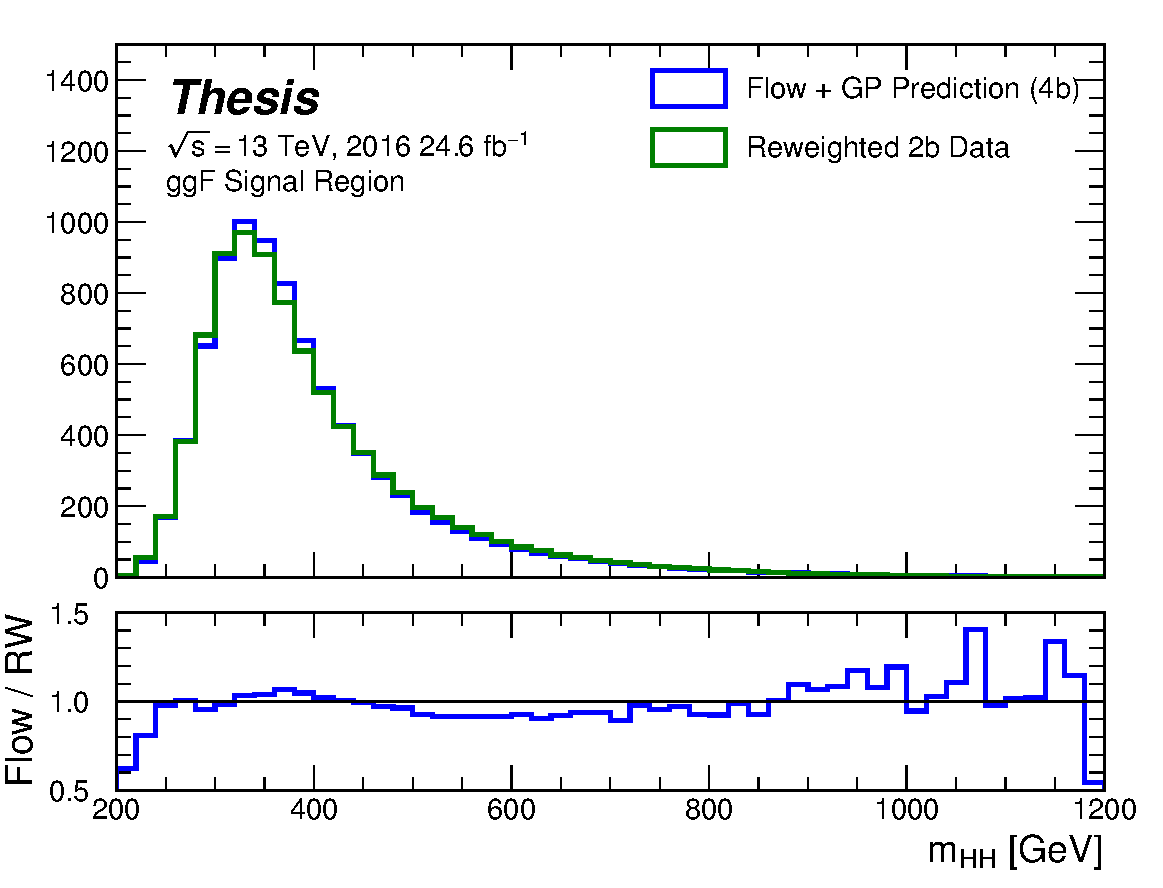
\includegraphics[width=0.48\textwidth]{figures/m-hh-comparison-flow-rw2b-16.pdf}
	}
	\subfloat{
	    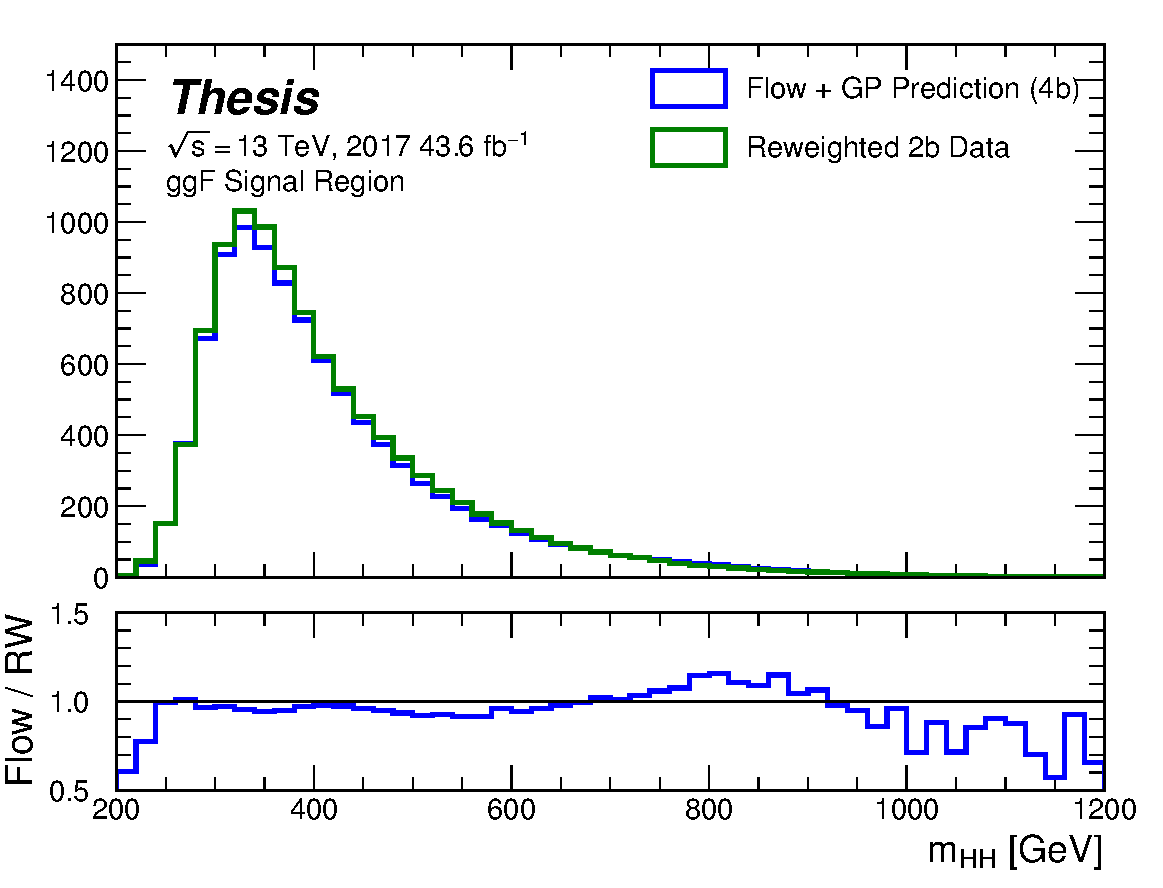
\includegraphics[width=0.48\textwidth]{figures/m-hh-comparison-flow-rw2b-17.pdf}
	}

	\subfloat{
	    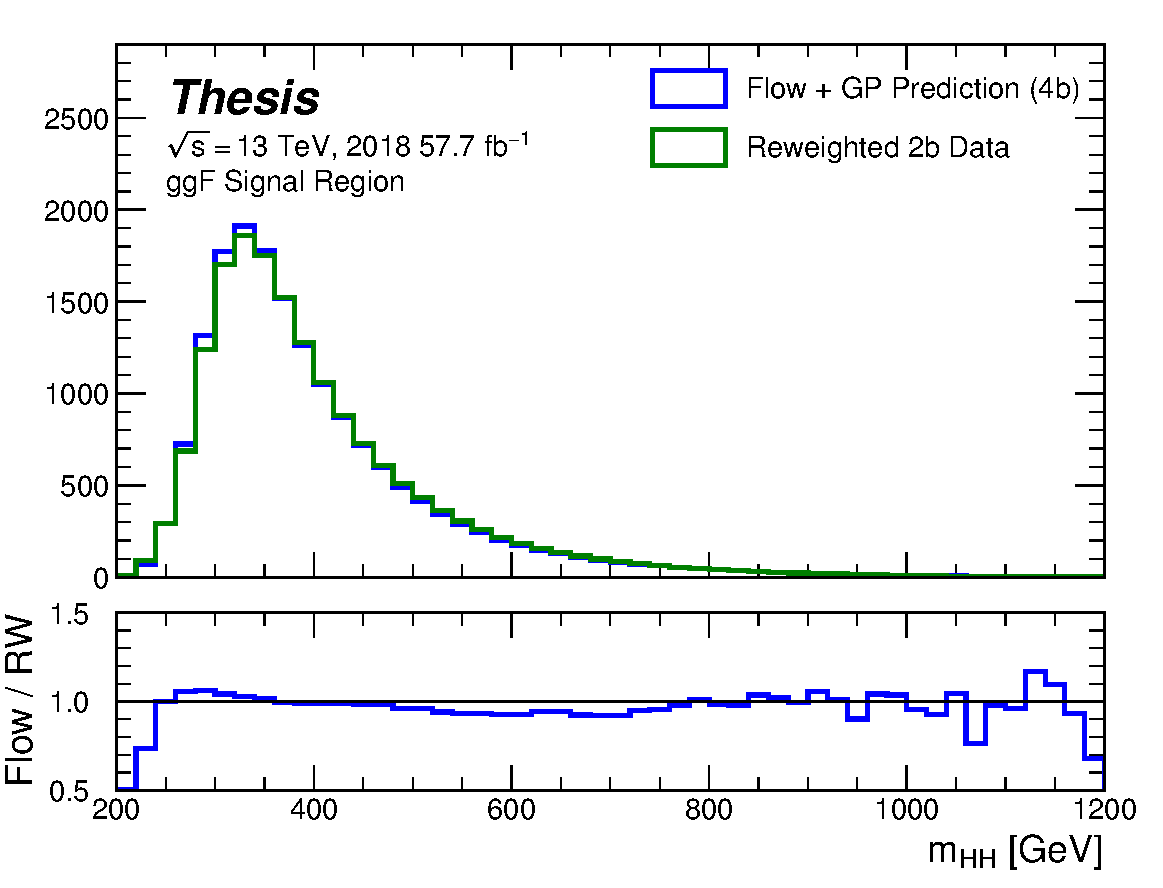
\includegraphics[width=0.48\textwidth]{figures/m-hh-comparison-flow-rw2b-18.pdf}
	}
	\caption{\label{fig:flow-gp-rw-4b} Comparison of the interpolation background estimate in the 
	$4b$ signal region with the control region derived reweighted 2b estimate, shown for each year 
	individually. Results are generally similar, within around 10~\%.}
\end{figure}

\subsection{Outstanding Points}
While good performance is demonstrated from the nominal interpolated background estimate, various 
uncertainties must be assigned according to the various stages of the estimate. These notably include
\begin{itemize}
	\item Assessing a statistical uncertainty on the normalizing flow training (cf. bootstrap uncertainty).
	\item Propagation of the Gaussian process uncertainty through the sampling procedure.
	\item Validation of the resulting estimate and assessment of necessary systematic uncertainties (e.g. from 
	validation region non-closure).
\end{itemize}
These are all quite tractable, but some, especially the choice of an appropriate systematic uncertainty, 
are certainly not obvious and require detailed study. In this respect, the reweighting validation work of the 
non-resonant analysis is certainly quite useful as a starting place in terms of the available regions 
and their correspondence to the nominal $4b$ signal region.


